%% 
%% Copyright 2007, 2008, 2009 Elsevier Ltd
%% 
%% This file is part of the 'Elsarticle Bundle'.
%% ---------------------------------------------
%% 
%% It may be distributed under the conditions of the LaTeX Project Public
%% License, either version 1.2 of this license or (at your option) any
%% later version.  The latest version of this license is in
%%    http://www.latex-project.org/lppl.txt
%% and version 1.2 or later is part of all distributions of LaTeX
%% version 1999/12/01 or later.
%% 
%% The list of all files belonging to the 'Elsarticle Bundle' is
%% given in the file `manifest.txt'.
%% 

%% Template article for Elsevier's document class `elsarticle'
%% with numbered style bibliographic references
%% SP 2008/03/01

\documentclass[preprint,12pt]{elsarticle}
    
    %% Use the option review to obtain double line spacing
    %% \documentclass[authoryear,preprint,review,12pt]{elsarticle}
    
    %% Use the options 1p,twocolumn; 3p; 3p,twocolumn; 5p; or 5p,twocolumn
    %% for a journal layout:
    %% \documentclass[final,1p,times]{elsarticle}
    %% \documentclass[final,1p,times,twocolumn]{elsarticle}
    %% \documentclass[final,3p,times]{elsarticle}
    %% \documentclass[final,3p,times,twocolumn]{elsarticle}
    %% \documentclass[final,5p,times]{elsarticle}
    %% \documentclass[final,5p,times,twocolumn]{elsarticle}
    
    %% For including figures, graphicx.sty has been loaded in
    %% elsarticle.cls. If you prefer to use the old commands
    %% please give \usepackage{epsfig}
    
    %% The amssymb package provides various useful mathematical symbols
    \usepackage{amssymb}

%\savesymbol{singleletter}								% American Mathematical Society symbols
\usepackage{float}												% customised float support
%\restoresymbol{X}{singleletter}
\usepackage{fancyhdr}											% improved header and footer support

\usepackage{amsmath}											% American Mathematical Society environments

\usepackage{epstopdf}
\usepackage{caption}
\usepackage{subcaption}
\usepackage{csvsimple}
\usepackage{booktabs} 
\usepackage{pifont}
\usepackage{flafter}

\usepackage{url}												% URL typesetting
\usepackage{texnames}											% BIBTeX, SliTeX, AMSTeX, PiCTeX and TeXsis logos
\usepackage{verbatim}											% multi-line comments
\usepackage{ifpdf}												% selective setup for PDF compilation	
\usepackage{algorithmicx}
\usepackage{longtable,tabu}
\usepackage{algcompatible}
\usepackage{algorithm}% http://ctan.org/pkg/algorithms
\usepackage{algpseudocode}% http://ctan.org/pkg/algorithmicx
\usepackage{breqn}
\usepackage{tikz}

\usetikzlibrary{shapes.geometric, arrows, decorations.text, fit}
\tikzstyle{process} = [rectangle, minimum width=3cm, minimum height=1cm, text centered, draw=black]
\tikzstyle{arrow} = [thick,->,>=stealth]
\tikzstyle{initial}=[circle,draw=black,text=black,text centered,minimum width=1cm,minimum height=1cm]

    %% The amsthm package provides extended theorem environments
    %% \usepackage{amsthm}
    
    %% The lineno packages adds line numbers. Start line numbering with
    %% \begin{linenumbers}, end it with \end{linenumbers}. Or switch it on
    %% for the whole article with \linenumbers.
    %% \usepackage{lineno}
    
    \journal{Applied Soft Computing}
    
    \begin{document}
    
    \begin{frontmatter}
    
    %% Title, authors and addresses
    
    %% use the tnoteref command within \title for footnotes;
    %% use the tnotetext command for theassociated footnote;
    %% use the fnref command within \author or \address for footnotes;
    %% use the fntext command for theassociated footnote;
    %% use the corref command within \author for corresponding author footnotes;
    %% use the cortext command for theassociated footnote;
    %% use the ead command for the email address,
    %% and the form \ead[url] for the home page:
    %% \title{Title\tnoteref{label1}}
    %% \tnotetext[label1]{}
    %% \author{Name\corref{cor1}\fnref{label2}}
    %% \ead{email address}
    %% \ead[url]{home page}
    %% \fntext[label2]{}
    %% \cortext[cor1]{}
    %% \address{Address\fnref{label3}}
    %% \fntext[label3]{}
    
    \title{Nature Inspired Algorithms for Prioritized Foraging}
    
    %% use optional labels to link authors explicitly to addresses:
    %% \author[label1,label2]{}
    %% \address[label1]{}
    %% \address[label2]{}
    
    \author{Jade Zo\"e Abbott}
    
    \address{}
    
    \begin{abstract}
    %% Text of abstract

    Foraging is a major problem in swarm robotics, which has been applied to many areas such as agriculture, and search and rescue. This dissertation defines a variation of swarm robotics foraging, called prioritized foraging. Prioritized foraging differs from other foraging problems, in that there are two types of items: prioritized items and non-prioritized items. Furthermore, a novel honey bee inspired foraging algorithm is developed. An empirical analysis of three foraging algorithms (a na\"ive algorithm, and two nature inspired algorithms, namely a desert ant inspired algorithm and the novel honey bee inspired algorithm) is performed on the prioritized foraging problem. The analysis investigates each algorithm's performance on the prioritized foraging problem in terms of the major swarm robotics characteristics of efficiency, scalability, flexibility, and robustness as well as the behaviours that enable those characteristics. The work concludes that the honey bee algorithm is highly efficient, highly flexible, highly scalable in terms of problem density, and most robust in terms of redundancy due to the algorithm's division of labour between prioritized and non-prioritized items. The desert ant algorithm is almost as efficient as the honey bee algorithm. The na\"ive algorithm has very poor efficiency, compared to the other algorithms, but was the most scalable in terms of swarm size. Both the desert ant and na\"ive algorithm experience poor flexibility, scalability in terms of problem density, and robustness in terms of redundancy.
    \end{abstract}
    
    \begin{keyword}
    %% keywords here, in the form: keyword \sep keyword
    
    %% PACS codes here, in the form: \PACS code \sep code
    
    %% MSC codes here, in the form: \MSC code \sep code
    %% or \MSC[2008] code \sep code (2000 is the default)
    Swarm Robotics, Foraging, Prioritized Foraging, Desert Ant, Honey bee
    
    \end{keyword}
    
    \end{frontmatter}
    
    %% \linenumbers
    
    %% main text
\section{Introduction}
\label{introduction}

\subsection{Motivation}
\label{motivation}

Consider a search and rescue mission after a natural disaster or mining accident. These search and rescue missions are usually extremely dangerous for the human rescuers who are deployed to search for survivors. The use of swarm robotics to perform such search and rescue mission has been proposed and explored as an alternative to using human rescuers \cite{murphy2008search,naghsh2008analysis}.

Swarm robotics is the co-coordination of large numbers of  relatively simple robots to perform a single collaborative function. Swarm robotics is inspired from the observation of social insects such as ants, termites, and bees \cite{dorigo2004swarm}. An important activity of all natural swarms is foraging for resources. Foraging is defined as the search and collection of resources from sources in an environment and returning the resources to a collection point \cite{winfield2009foraging}. These resources could be food, water, or building materials. Foraging is an abstraction of the search and rescue problem where the trapped humans are items that robots need to locate and remove to a safe location. 

In a search and rescue mission, the location of trapped humans is usually unknown and humans can be potentially be blocked by rubble, which needs to be removed before the humans can be safely removed. A swarm of robots would need to search for the humans, as fast as possible, to avoid further danger, injury or loss of life. If robots cannot locate the humans, they will have to begin clearing debris in the hope of locating them, as well as clearing the route between the trapped humans and the safe zone. Locating and removing the humans is prioritized above removal of the debris, but often the debris must be removed, in order to locate the trapped humans. Thus there exists a resource prioritization from the perspective of the robot.

Resource prioritization is also relevant in mining problems where the metal ore is prioritized and the waste rock should be cleared to better access the valuable ore. In common gold mining techniques, the ore and waste rock are collected and transported to the surface and chemical techniques are used to separate them. The transport of the waste rock (which forms the majority of the load) to the surface is extremely expensive, so there is a cost benefit to separate the ore and the waste rock beneath the surface and transport only the valuable ore to the surface.

The above search and rescue problem and mining problem can be abstracted as a foraging problem where there exist resources with differing priorities. In the case of search and rescue, the humans are the prioritized resource and the debris is the non-prioritized resource. In mining, the ore is the prioritized resource and the waste rock is the non-prioritized resource. 

In nature, in times of stress, the collection of one resource may be prioritized over others - such as water during a drought or food before winter. Individuals in a natural swarm often adapt behaviour appropriately to enable greater collection of the prioritized item.

This study defines the prioritized foraging problem, and proposes three swarm robotics foraging algorithms to be evaluated on the prioritized foraging problem. The study proposes metrics to evaluate each algorithm's performance on the prioritized foraging problem in terms of foraging efficiency, flexibility, scalability and robustness. The algorithms are developed in a simulated environment. Each algorithm's performance is evaluated on environments of a variety of complexities, with various swarm configurations.



\subsection{Foraging in Nature}
\label{foraginginnature}
As with many swarm robotics problems, the inspiration for foraging comes from nature, in particular, social insects such as ants and honey bees. This section describes the biological inspiration for foraging. Section~\ref{biological:ants} describes foraging in ants, while foraging activities of bees are discussed in Section~\ref{bees:biologicalinspiration}. Section~\ref{foraging:other} discusses other types of foraging techniques seen in nature.


\subsubsection{Ant Foraging Behaviour}
\label{biological:ants}
% Intro 
As with many swarm robotics problems, the inspiration for foraging comes from nature, in particular, social insects such as ants and honey bees. This section describes the biological models that are used in the algorithms derived by this thesis. 

%Ants
The study of ants has revealed that impressive emergent activities can be achieved with simple interacting agents with only a few simple rules. Many ant species use a form of communication known as stigmergy \cite{dorigo2000ant}. Ants perform indirect communication between ants by depositing a substance known as pheromone. In foraging, pheromone is deposited on the paths between the nest and the food source. Other ants detect the deposited pheromone and will prefer to follow paths which have a greater amount of pheromone deposit. Ant pheromones have been modelled in numerous swarm intelligence algorithms such as ant systems \cite{dorigo2006ant, dorigo2010ant}. 
 
Although algorithms based on ant foraging behaviour are used to solve optimization problems, the algorithms are often difficult to replicate in a real-life robot environment, since most of the algorithms need to model pheromone dropping and detection. A robotics algorithm that uses pheromone requires robots to be equipped with a substance-distributors, beacon-deployers or complex communication that simulates pheromone deposition and trail-following \cite{hoff2010two}.

The desert seed-harvester ant (\textit{Pogonomyrmex ant}) does not make use of stigmergy to forage, because pheromone deposited on desert sand would be blown away by the wind \cite{collett1992visual,hecker2015beyond}. Instead, desert ants use a technique called path integration for navigation to relocate food sources that have already been found by random exploration \cite{collett1998local,wehner2003desert}. Fig~\ref{pathintegration} demonstrates path integration. The black solid lines represent the path of the ant and the blue dotted lines show how the direction to the nest is maintained as the ant explores. The ant is constantly monitoring the change in heading from the original heading such that, at the destination, the ant has a direction directly back to the sink. As a result, a shortcut back to the nest is calculated in order to minimize the heat stress caused by walking through the hot desert. The shortcut back to the nest is known as the home vector \cite{muller1988path}. Path integration, more commonly known as dead reckoning, is a key evolutionary aspect gained from living in the hot barren desert. When path integration fails, the ant resorts to using landmarks, such as the sun, for navigation \cite{collett1998local}.

\begin{figure} [h]
	\centering
	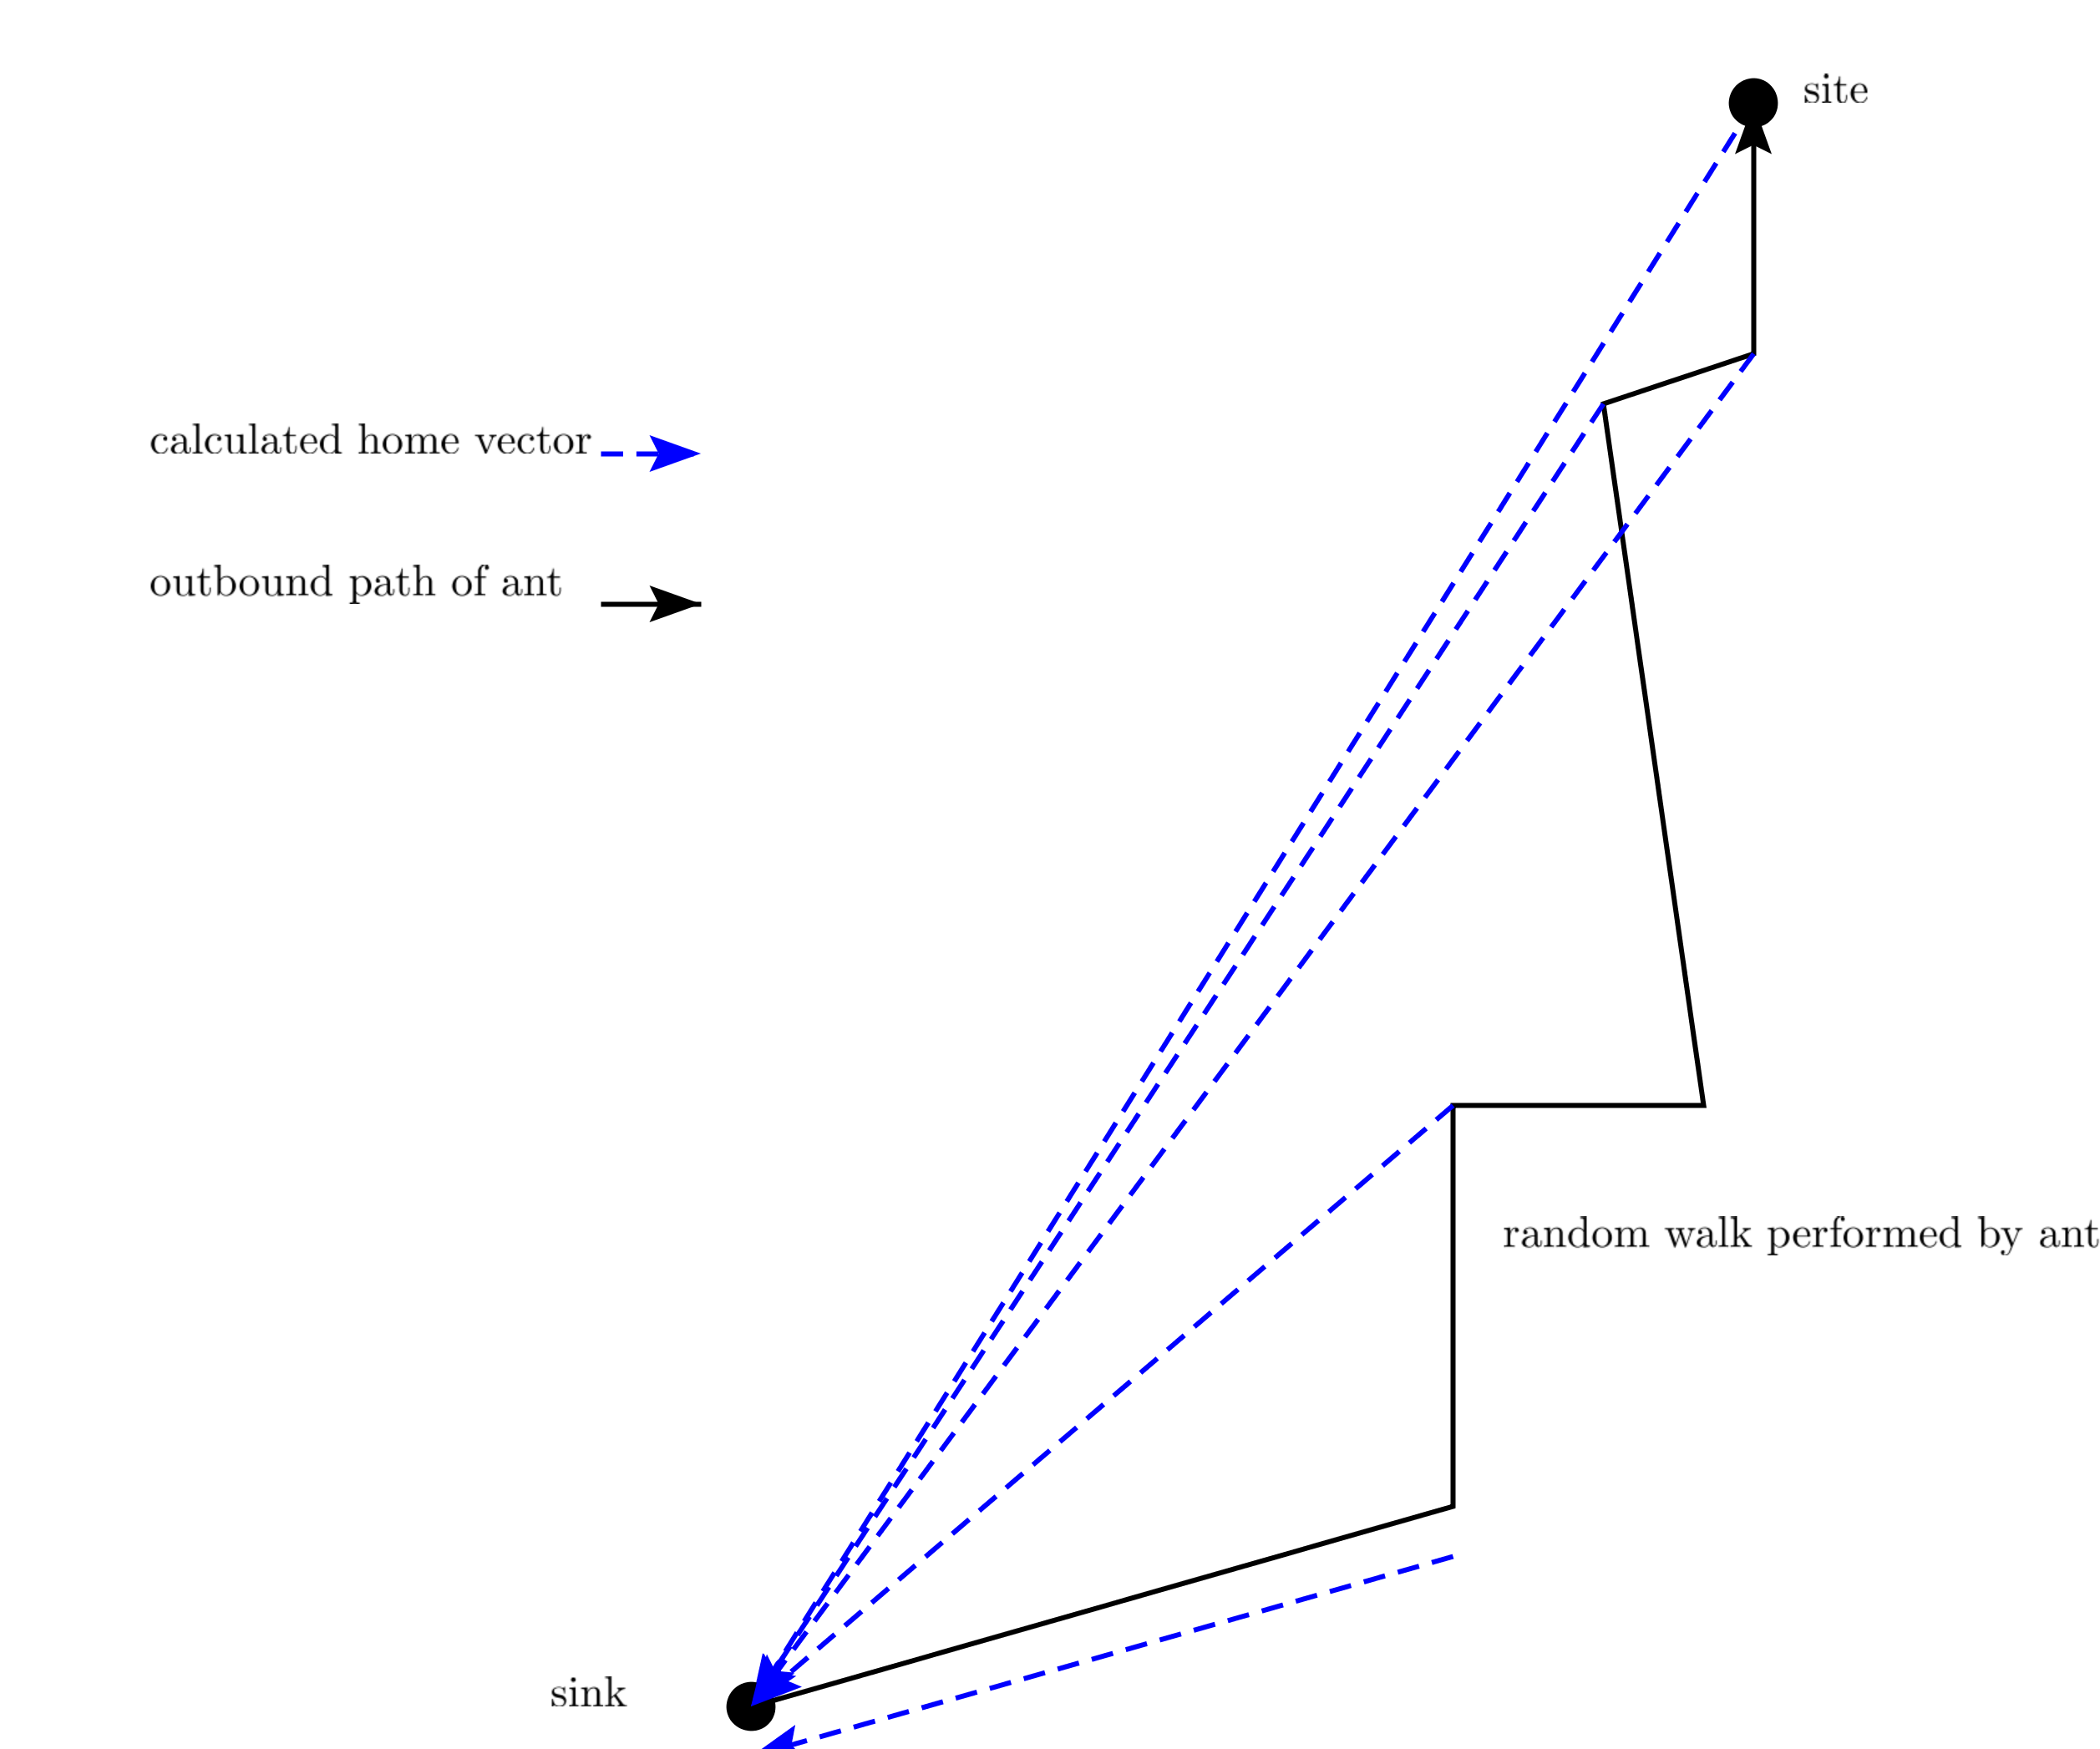
\includegraphics[width=\textwidth]{figures/drawing.png}
	\caption{Path Integration}
	\label{pathintegration}
\end{figure}

Due to the lack of pheromone, the desert seed-harvester ant was simpler to model for real-robot interaction. Desert seed-harvester ant foraging has been modelled in \cite{moller1998modeling,hecker2012formica}. Hecker \textit{et al} \cite{hecker2012formica} performed experiments to compare the performance of two foraging algorithms: The one algorithm was based on desert ant foraging which has no pheromone-like communication and the other algorithm included pheromone-like communication. It was shown that communication improved performance; however, the desert ant based algorithm still performed comparatively well. 

\subsubsection{Bee Foraging Behaviour}
\label{bees:biologicalinspiration}
Bees have an impressive set of abilities considering the simplicity of a single individual. They have the ability to remember the colour and shape of flowers \cite{zhang2006honeybee}, and in terms of navigation, they are able to learn local features and routes due to well-developed learning and memorizing capacities \cite{menzel2001cognitive}. Honey-bees are even time aware \cite{moore1989influence}. 

Honey bees have efficient division of labour between different functions in the hive, such as foraging and brood-care. Within the foraging activity itself, honey bees perform foraging-specific division of labours. Honey bee foraging is made up of three different roles namely employed foraging, unemployed foraging and scouting \cite{seeley2009wisdom}. Scouts explore the environment to locate new food sources. Once a source has been found, scouts return to the hive to communicate information about the located food source. To communicate the foraging information, scout bees perform a waggle-dance at the hive. The waggle-dance communicates information about the distance and bearing of the resource. Recruitment \cite{seeley2009wisdom} refers to the process of communicating high quality foraging sites to the swarm.

Unemployed foragers wait on the dance floor, and evaluate the dances of the scout bees. An unemployed bee selects a location described by the scout bees, and become an employed forager. Employed forager bees use the information about the resource, attempt to locate the source, load themselves with food, and return to the hive where unemployed foragers are ready to offload the food. Jansen \cite{janson2007searching} suggests that unemployed bees become exploring scouts when they do not detect any dancing scout bees. 



%TODO Literature Review 
\subsection{Prioritized Foraging}
\label{Prioritized Foraging}

%TODO: insert citation
The prioritized foraging problem, illustrated in Fig.\ref{prioritizedforaging}, is a modified version of the multi-foraging problem. In prioritized foraging, an environment has two types of items: prioritized items and non-prioritized items. The goal is to forage all the items of the prioritized type. The possibility exists that prioritized items become trapped among non-prioritized items and thus the non-prioritized items need to be removed from the environment to clear an access route to the prioritized items. 


The prioritized foraging problem has increased difficulty compared to traditional multi-foraging problems, due the fact that foraging the non-prioritized item more than required will result in a waste of time and energy. The goal of research in prioritized foraging is to develop an algorithm to efficiently adapt the number of robots searching for prioritized items to those moving non-prioritized items out the way. 


The prioritized foraging problem has similarities to the problem of search and rescue. For example, in the case of a collapsed building, robots will need to get to the survivors as quickly as possible. However, it is important that some robots move waste material in order to reach the trapped survivors. Prioritized foraging could be applied to the gold mining problem where gold needs to be foraged as a priority, and waste needs to be moved out of the way.

\begin{figure} [h]
	\centering
	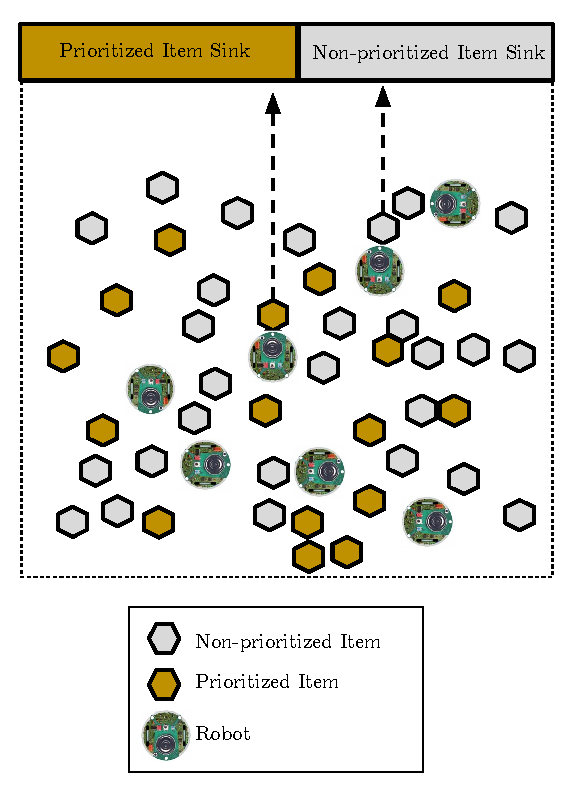
\includegraphics[width=0.65\textwidth]{figures/EpuckGoldMining2.pdf}
	\caption{Prioritized Foraging Problem }
	\label{prioritizedforaging}
\end{figure}

The prioritized foraging problem has the following characteristics: The environment has a bounded search space, with multiple source areas for items which can be placed in multiple sinks. Multiple object types exist in the environment - the prioritized items and the non-prioritized items. The primary  performance measure for the prioritized foraging problem is time, in terms optimizing the time taken to forage each type of item. 


\section{Algorithms}
\label{algorithms}


\section{Na\"ive foraging algorithm}
\label{naiveforaging}

Na\"ive foraging consists of the following tasks: searching for an item, grabbing an item, returning home with the item, and storing the item at the sink. The steps performed by the algorithm are illustrated in Figure~\ref{naiveforagingstatediagram}, and described below:  

\begin{enumerate}
	\item Robots perform a random walk until they find an item.
	\item On locating an item, the robot grips the item. If the item has been moved before the robot is able to pick it up, the robot will continue to explore; otherwise, the robot returns the item to the correct sink using a beacon-based homing algorithm.
\end{enumerate}

\begin{figure} [h]
	\centering
	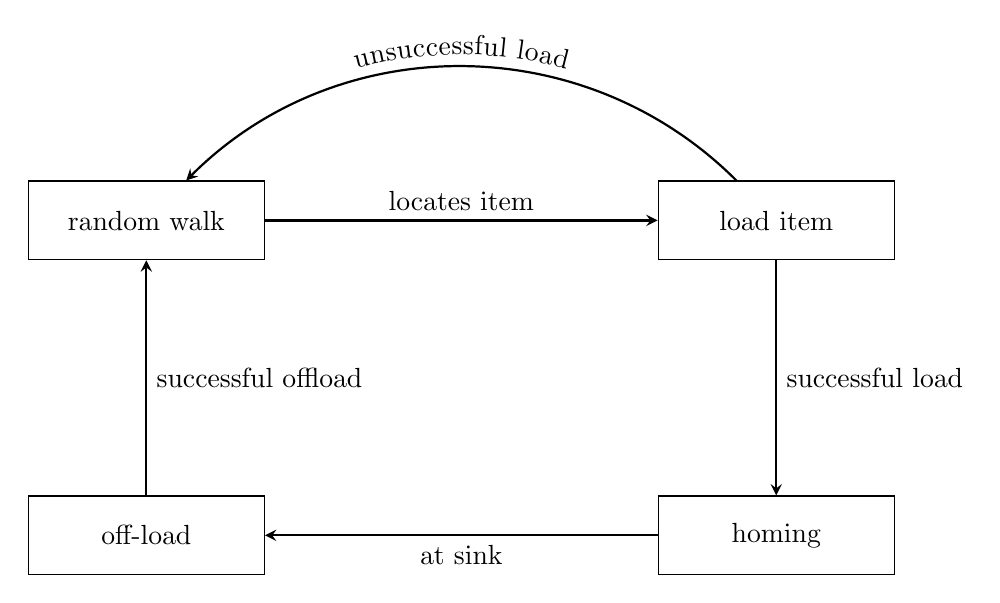
\begin{tikzpicture}[node distance=8cm]
	\node (randomwalk) [process] {random walk};
	\node (offload) [process, below of=randomwalk, yshift=4cm] {off-load};
	\node (loaditem) [process, right of=randomwalk] {load item};
	\node (homing) [process, right of=offload] {homing};
	\draw [arrow] (randomwalk) -- node[anchor=south] {locates item} (loaditem);
	\draw [arrow] (loaditem) -- node[anchor=west] {successful load} (homing);
	\draw [arrow] (homing) -- node[anchor=north] {at sink} (offload);
	\draw [arrow] (offload) -- node[anchor=west] {successful offload} (randomwalk);

	\draw[arrow,postaction={decorate,decoration={text along path,reverse path,raise=1ex,text align=center,text={unsuccessful load}}}] (loaditem) to[bend right=45] (randomwalk);
	\end{tikzpicture}
	\caption{Nai\"ve Foraging State Diagram}
	\label{naiveforagingstatediagram}
\end{figure}

Na\"\i ve foraging includes only the most minimal set of foraging actions and is included as a baseline for comparison to evaluate how novel techniques, such as the desert-ant foraging or honey-bee foraging, compare to a standard model \cite{ostergaard2001emergent,hoff2010two}.

The following random walk is used: A robot chooses a random direction, $\sigma$, and a random distance, $m\in(0,M)$, where $M$ is a chosen maximum path length. The robot walks in direction $\sigma$ for distance $m$, or until the robot reaches a boundary. The robot then chooses new values for $\sigma$ and $m$.


\section{Desert ant foraging}
\label{desertantforaging}


As discussed in Section~\ref{biological:ants}, desert ant foraging behaviour is a very suitable model for robot foraging, since no pheromone depositors or pheromone mimickry is required. Pheromone depositors or pheromone mimickry are quite complex to perform in robot environments. Instead of pheromone, desert ants use path integration (PI) to memorize the location of an existing food source and later to return to the memorized source to find more food, as discussed in Section~\ref{biological:ants}. The notion of returning to a previously explored site is known as site fidelity \cite{switzer1993site}. The desert ant algorithm does not require communication between robots or the dispersal of beacons, and is thus simpler than many other swarm robotic foraging algorithms. The desert ant algorithm was defined by Hecker \textit{et al} \cite{hecker2012formica}. The desert ant foraging robots can be in the following states:

\begin{enumerate}
	\item\textbf{Exploration State}: A robot in the exploration state performs a random walk with PI. The random walk used is the same random walk as discussed in Section~\ref{naiveforaging}. The purpose of the exploration state is to explore the environment to locate items. 
	\item\textbf{Loading State}: On finding an item, the robot switches into the loading state. In the loading state, the robot loads the item and memorizes the current PI vector. The PI vector is memorized so that the robot can use it to return to the sink and then later to return to the site where the item was found. If loading of the item fails (perhaps due to another robot loading the item), then the robot returns to the exploration state; otherwise, the robot moves into the homing state.
	\item\textbf{Homing State}: In the homing state, the robot uses the PI vector to move to the sink. The use of the PI vector will enable the robot to follow the most direct route back to the sink.
	\item\textbf{Offloading State}: When the robot arrives at the sink, the robot switches into the offloading state, where the robot simply offloads the item into the sink. 
	\item\textbf{Locating State}: Once the robot has offloaded the item, the robot switches to the locating state. In the locating state, the robot follows the memorized PI vector to the location of the previous item. The premise of returning to the site where the previous item was found is that more items may exist where the previous item was located in order to locate more items. If another item is found, the robot moves into the loading state; otherwise, the robot returns to the exploration state in the search of new items. 
\end{enumerate}

All robots begin at random positions adjacent to the sink in the exploration state. The desert ant foraging states and transitions are illustrated in Figure~\ref{fig:desertantstate}.

\begin{figure} [h]
	\centering
	\begin{tikzpicture}[node distance=6cm]
	\node (explorationstate) [process] {explore};
	\node (loadstate) [process, right of=randomwalk] {loading};
	\node (homing) [process, below of=loadstate,yshift=2cm] {homing};
	\node (offload) [process, left of=homing] {offload};
	\node (locating) [process, left of=explorationstate] {locating};
	\draw [arrow] (explorationstate) -- node[anchor=south] {locates item} (loadstate);
	\draw [arrow] (loadstate) -- node[anchor=west] {successful load} (homing);
	\draw [arrow] (homing) -- node[anchor=south] {at sink} (offload);
	\draw [arrow] (offload) -- node[anchor=east] {offload complete} (locating);
	\draw [arrow] (locating) -- node[anchor=south] {item not found} (explorationstate);
	\draw[arrow,postaction={decorate,decoration={text along path,raise=1ex,text align=center,text={locates item}}}] (locating) to[bend left=45] (loadstate);
	\draw[arrow,postaction={decorate,decoration={text along path,reverse path, raise=1ex,text align=center,text={unsuccessful load}}}] (loadstate) to[bend left=45] (explorationstate);
	\end{tikzpicture}
	\caption{Desert Ant Foraging State Diagram}
	\label{fig:desertantstate}
\end{figure}

	
%%%%%%%%%%%%%%%%%%%%%%%%%%%%%%%%%%%%%%%%%%%%%%%%%
%%%%%%%%%%%%%%%%%%%%%%%%%%%%%%%%%%%%%%%%%%%%%%%%%

\section{Honey bee foraging}
\label{honeybeeforaging}
%TODO Describe the 3 states referring back to where they were discussed in the previous section.

The honey bee foraging algorithm presented in this section is based on the foraging behaviour of honey bees as described in Section~\ref{bees:biologicalinspiration}. The algorithm described requires robots to take on one of three roles, namely, scout robots, unemployed forager robots, or employed forager robots. The roles of the robots and the transitions to and from these roles are described in this section. 

Figure~\ref{honeybeestate} provides a simplified diagram for the honey bee prioritized foraging algorithm, illustrating the roles and the transitions between each role and the states within these roles. The dance and explore states of the scout robots are shown separately for clarity and the employed forager states are outlined separately in Figure~\ref{employedforagerstatediagram}.

To more succinctly define the honey bee prioritized foraging algorithm, the algorithms for each behavioural state, within each role, are provided below. For each algorithm, note that the current state of the robot is denoted $state$, and the $state$ is modified during the behaviour to denote the next state of the robot. The current time step is denoted as $i$. The algorithm for a single state is executed once per time step $i$.

\begin{figure}[h]
	\centering
	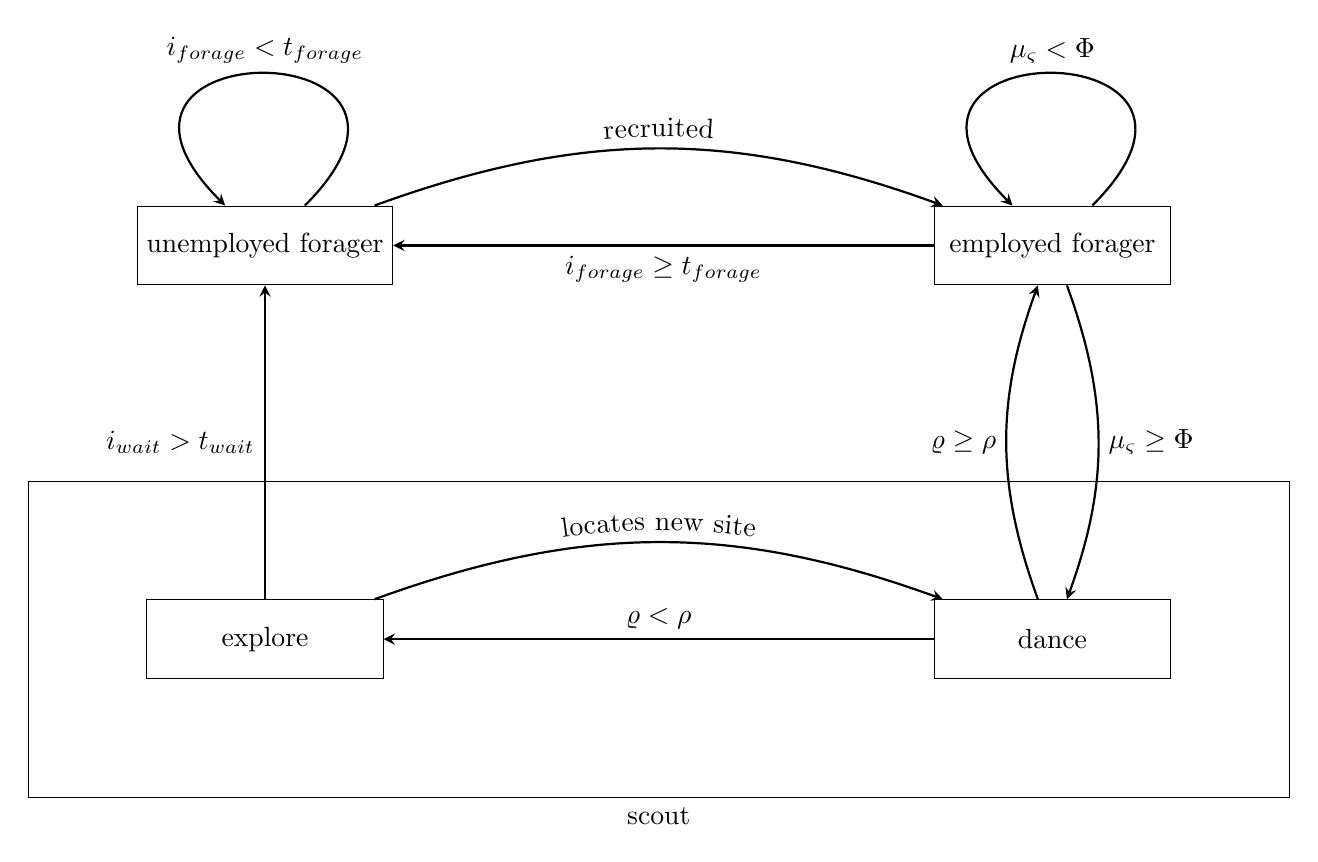
\begin{tikzpicture}[node distance=10cm]
	\node (wait) [process] {unemployed forager};
	\node (forage) [process, right of=wait] {employed forager};
	\node (dance) [process, below of=forage,yshift=5cm] {dance};
	\node (scout) [process, left of=dance] {explore};
	
	\draw [arrow,postaction={decorate,decoration={text along path,raise=1ex,text align=center,text={recruited}}}] (wait) to[bend left=20] (forage);
	
	\draw [arrow] (forage) -- node[anchor=north] {$i_{forage} \geq t_{forage}$} (wait);
	
	\draw [arrow] (forage) to[bend left=20] node[anchor=west] {$\mu_\varsigma \geq \Phi$} (dance);
	\draw[arrow] (dance) to[bend left=20] node[anchor=east] {$\varrho \geq \rho$} (forage);
	\draw [arrow] (dance) -- node[anchor=south] {$\varrho < \rho$} (scout);
	\draw [arrow] (scout) -- node[anchor=east] {$i_{wait} > t_{wait}$} (wait);
	\draw [arrow,postaction={decorate,decoration={text along path,raise=1ex,text align=center,text={locates new site}}}] (scout) to[bend left=20] (dance);
	\draw [arrow] (forage) to[loop] node[anchor=south] {$\mu_\varsigma < \Phi$} (forage);
	\draw [arrow] (wait) to[loop] node[anchor=south] {$i_{forage} < t_{forage}$} (wait);
	\node[process, fit=(scout)(dance), inner sep=1.5cm, label={270:scout}] (all) {};
	\end{tikzpicture}
	\caption{Honey Bee Foraging State Diagram}
	\label{honeybeestate}
\end{figure}

Section~\ref{scoutrobots} presents the behaviour of scout robots, while the behaviour of forager robots is described in Section~\ref{foragerrobots}. The initial state of the swarm is described in Section~\ref{initialstates}, while Section~\ref{natureinspired:divisionoflabour} describes the division of labour mechanism used by the honey bee algorithm.

\subsection{Scout Robots}
\label{scoutrobots}
Scout robots mimic the scouting behaviour of the scout honeys bees as discussed in Section~\ref{bees:biologicalinspiration}. The purpose of the scout honey bees is to locate high quality sites of resources. If the discovered site is of a high enough quality, then the scout will broadcast the location of the site to the unemployed forager robots at the sink. 

Each scout robot begins in the explore state where the scout robot performs a random walk. Algorithm~\ref{algorithm:explore} provides a step-by-step explanation of the explore state of the scout robot. Variable $\varsigma$ saves the robot's item specialization as prioritized or non-prioritized. The random walk performed is the same random walk as discussed in Section~\ref{naiveforaging}. As the scout robot moves, the robot maintains a PI vector $v$ as explained in Section~\ref{biological:ants}. Upon finding an item $\vartheta$ of type $\varsigma$ at site $\xi$, the robot loads the item and then performs an evaluation of the quality, $\mu_\varsigma$, of the site $\xi$ for the item type $\varsigma$. 


% Scout algorithms
\begin{algorithm}
\caption{Explore State of Scout Robot}
\label{algorithm:explore}
\begin{algorithmic}[1]
\Function{explore}{$role, state, v, \varsigma, i$}
%move random direction from location l
\State \text{perform a single random walk step from the current location}
\State \text{update path integration vector $v$}

\If {\text{item $\vartheta$ of priority $\varsigma$ is detected in vicinity}}
 	\State \text{calculate quality $\mu_\varsigma$ of site $\xi$ }
	\State {$\omega \gets v$}
	\State load item $\vartheta$
\ElsIf {$i_{explore} > f_{max}$ and $i_{explore} \leq t_{explore}$}
	\State $\varsigma \gets N$
\ElsIf {$i_{explore} > t_{explore}$}
	\State $state \gets homing$
\EndIf
\State $i = i + 1$
\EndFunction
\end{algorithmic}
\end{algorithm}

The quality, $\mu_\varsigma$, of site $\xi$, for a robot scouting items of type $\varsigma$ is calculated as the estimated density of items of type $\varsigma$ in the local vicinity of the found item $\vartheta$. The robot has distance sensor values $k_j\in[0,1]$ for $j = 1,...,n$, where $n$ is the number of distance sensors. A distance sensor reading of 0 means that nothing is detected in the sensor's range and a distance sensor reading of 1 indicates that the robot is touching an item. The sensor value $k_j$ for item type $\varsigma$, denoted $k_{j_\varsigma}$, is calculated as 
\begin{equation}
\label{densitytype}
k_{j_\varsigma}=
    \begin{cases}
      k_j & \text{if detected item is type $\varsigma$} \\
      0 & \text{otherwise}
    \end{cases}
\end{equation}

The site quality of type $\varsigma$, $\mu_\varsigma$, is calculated using
\begin{equation}
\label{density}
\mu_\varsigma = \frac{1}{n}\sum\limits_{x=1}^n k_{x_\varsigma}
\end{equation}
 
Before returning to the sink with the item, the scout memorizes the PI vector $v$ in site location variable $\omega$. The scout robot then switches to the homing state given in Algorithm~\ref{algorithm:scout:homing}. Using PI vector $\omega$, the scout returns the item $\vartheta$ to the sink. When the scout robot has returned to the sink, $S_\varsigma$, the scout robot offloads the item $\vartheta$. If the quality $\mu_\varsigma$ of the visited site $\xi$ is larger than site quality threshold, $\Phi$, the scout robot switches into the dance state, which is summarized in Algorithm~\ref{algorithm:recruit}. If the quality, $\mu_\varsigma$, of the visited site $\xi$ is less than site quality threshold, $\Phi$, the robot takes on the role of an employed forager and switches into the locate state, as outlined in Algorithm~\ref{algorithm:employedforager:locating}.


\begin{algorithm}
\caption{Homing State of Scout Robot}
\label{algorithm:scout:homing}
\begin{algorithmic}[1]
\Function{scout homing}{$role, state, v, \varsigma, i, \omega$}
\If {\text{robot is at sink $S_\varsigma$ and robot is loaded}}
	\State \text{robot offloads item $\vartheta$}
	\If {\text{$\mu_\varsigma > \Phi \text{ and } \varsigma = \text{prioritized}$}}
		\State \text{$state \gets dance$}
	\Else 
		\State \text{$role \gets \text{employed forager}$}
		\State \text{$state \gets locate$}
	\EndIf
\Else
	\State{\text{calculate direction $\sigma$ to sink $S_\varsigma$ from current location}}
	\If{\text{robot can move in direction $\sigma$}}
		\State \text{robot moves a step in direction $\sigma$}
	\EndIf
\EndIf
\State $i =i + 1$
\EndFunction
\end{algorithmic}
\end{algorithm}


\begin{algorithm}
\caption{Dance State of Scout Robot}
\label{algorithm:recruit}
\begin{algorithmic}[1]
\Function{dance}{$role, state, v, \varsigma, i, \omega, \mu_\varsigma$}
\If {$i_{dance} < t_{dance}$}
	\State \text{broadcast $\omega$ and $\mu_\varsigma$ to robots at the sink} 
\Else 
	\State \text{$\varrho = random(0,1)$}
	\If {$\varrho < \rho$} 
		\State{$role \gets \text{employed forager}$}
		\State{$state \gets locate$}
	\Else
		\State{$state \gets explore$}
	\EndIf
\EndIf
\State $i =i + 1$
\EndFunction
\end{algorithmic}
\end{algorithm}

% Employed Forager
\begin{algorithm}
\caption{Locate State of Employed Forager}
\label{algorithm:employedforager:locating}
\begin{algorithmic}[1]
\Function{forage}{$role, state, v, \varsigma, i, \omega, \mu_\varsigma$}
	\State \text{get direction $\sigma$ using path integration vector $\omega$}
	\State \text{robot moves a step in direction $\sigma$}
	\If {\text{(robot has finished path integration) OR (robot can see item of type $\varsigma$)}}
		\State $state \gets load$
	\EndIf
	\State $i =i + 1$
\EndFunction
\end{algorithmic}
\end{algorithm}

In the dance state, the scout robot communicates the location, $\omega$, and quality, $\mu_\varsigma$, of the previous site, $\xi$, to the unemployed workers at the sink. The communication is akin to the waggle dance performed by honey bees in nature, as discussed in Section~\ref{bees:biologicalinspiration}. A scout robot's ``dance" takes the form of a localized broadcast communication between the scout and the unemployed forager robots near the sinks. The scout robot communicates the site quality and location for the unemployed foragers for $t_{dance}$ time steps.

After the scout robot has completed broadcasting site details to the unemployed foragers, the scout robot must decide to either stay a scout robot and switch back to the explore state, or to become an employed forager robot and begin foraging the previous site. The scout robot becomes an employed forager robot with probability of $\rho$. If a random number $\varrho\in[0,1]$ is selected such that $\varrho$ is less than $\rho$, then the scout robot remains a scout and begins to explore the environment. If $\varrho$ is greater than or equal to $\rho$ then the scout becomes an employed forager. Increasing the site quality threshold, $\rho$, will make the scout robots more selective about the sites they broadcast. Decreasing $\rho$ will result in scout robots being less selective about the sites they broadcast.

\subsection{Forager Robots}
\label{foragerrobots}

There are two types of forager robots: The unemployed foragers and employed foragers. The unemployed forager robots take on the role of unemployed foragers from foraging honey bees discussed in Section~\ref{bees:biologicalinspiration}. Unemployed forager robots remain at the sink and await dance behaviour from a scout robot. This wait state is described in Algorithm~\ref{algorithm:unemployedforager:locating}.

\begin{algorithm}
\caption{Wait State of Unemployed Forager}
\label{algorithm:unemployedforager:locating}
\begin{algorithmic}[1]
\Function{wait}{$state, v, \varsigma, i, \omega, \mu_\varsigma$}
\If {$i_{wait} \geq t_{wait}$}
	\State{$role \gets scout$}
	\State $\varsigma \gets P$
	\State{$state \gets explore$}
\ElsIf {\text{scout robot is broadcasting at sink}}
	\State \text{receive site location $\omega$ and site quality $\mu_\varsigma$}
	\State $role \gets \text{employed forager}$
	\State $state \gets locate$
\EndIf
\State $i =i + 1$
\EndFunction
\end{algorithmic}
\end{algorithm}

A scout robot dances at the sink after locating an item $\vartheta$ at some site $\xi$. Each unemployed forager decides whether to listen to the scout robot with a probability of $\alpha$. If an unemployed forager robot chooses to accept the details communicated by the scout, then the unemployed foraged robot has been recruited and becomes an employed forager robot. The unemployed forager takes on the same item specialization, $\varsigma$, as the dancing scout robot. The unemployed forager will thus only search for items of type $\varsigma$. 

The employed forager robots are modelled based on the employed forager bees as discussed in Section~\ref{bees:biologicalinspiration}. The purpose of the employed forager robot is to forage the sites communicated by scout robots. When an unemployed forager robot takes on the role of an employed forager robot after recruitment by a scout robot, the employed forager starts in the locate state, described in Algorithm~\ref{algorithm:employedforager:locating}. In the locate state, the employed forager robot uses the PI vector $\omega$ to relocate the site $\xi$. Once the site $\xi$ has been relocated, the employed forager robot switches into the load state, as described in Algorithm~\ref{algorithm:loading}. If an item $\vartheta$ of type $\varsigma$ is detected in the vicinity of the located site, then the item is loaded. After successfully loading the item, the robot switches to the homing state. If the employed forager robot does not detect an object in the vicinity of the site $\xi$, then the employed robot switches to the local search state in order to perform a brief local search for items nearby. 

\begin{algorithm}
\caption{Load State of Employed Forager}
\label{algorithm:loading}
\begin{algorithmic}[1]
\Function{loading}{$role, state, v, \varsigma, i, \omega, \mu_\varsigma$}
\If {\text{item $\vartheta$ of priority $\varsigma$ is detected in vicinity}}
	\State \Call{load}{$\vartheta$}
	\State{$state \gets homing$}
\Else
	\State{$state \gets local\_search$}
\EndIf
\EndFunction
\end{algorithmic}
\end{algorithm}

The local search is performed for a limited number of time steps, $t_{ls}$. At each time step, $i_{ls}$, the robot checks if an item of priority $\varsigma$ is nearby and if the item can be loaded. If an item $\varsigma$ can be loaded, then the robot loads the item and switches to the homing state. If the employed forager robot can see an item $\varsigma$, but it is not close enough to be loaded, then the robot moves in the direction of the item. If the employed forager can not see an item in the vicinity, then the robot moves in a random direction, $\sigma$. The local search state is summarized in Algorithm~\ref{algorithm:employedforager:localclustersearch}. If $i_{ls}$ is greater than $t_{ls}$, then the foraging site is depleted and so the employed forager robot must return to the sink without an item.

\begin{algorithm}
\caption{Local Search State of Employed Forager}
\label{algorithm:employedforager:localclustersearch}
\begin{algorithmic}[1]
\Function{local\_search}{$role, state, v, \varsigma, i, \omega, \mu_\varsigma$}
\If {\text{$i_{ls} < t_{ls}$}}
		\If {\text{item $\vartheta$ of priority $\varsigma$ is nearby and can be loaded}}
			\State \Call{load}{$\vartheta$}
			\State{$state \gets homing$}	
		\ElsIf {\text{item $\vartheta$ of priority $\varsigma$ can be seen but is not close enough}}
			\State \text{select direction $\sigma$ to move towards item $\vartheta$}
			\State \text{robot moves a step in direction $\sigma$}
		\Else
			\State \text{select a random direction $\sigma$}
			\State \text{robot moves a step in direction $\sigma$}	
		\EndIf
\Else
	\State{$state \gets homing$}
\EndIf
\State $i =i + 1$
\EndFunction
\end{algorithmic}
\end{algorithm}

When in the homing state, the employed forager robot moves towards the appropriate sink, $S_\varsigma$, in order to off-load item $\vartheta$. Once at sink $S_\varsigma$, if the employed forager robot is loaded, it offloads the item and switches back to the locate state and thus repeats the steps of foraging the site $\xi$. If the employed forager robot is not loaded, the employed forager robot takes on the role of an unemployed forager and switches into the wait state. The reason for switching from an employed forager to an unemployed forager is because an item could not be found at the site $\xi$, and the site has likely been depleted. Thus the employed forager switches to an unemployed forager in order to await recruitment by a scout robot.

\begin{algorithm}
\caption{Homing State of Employed Forager Robot}
\label{algorithm:forager:homing}
\begin{algorithmic}[1]
\Function{employed forager homing}{$role, state, v, \varsigma, i, \omega$}
\If {\text{robot is at sink $S_\varsigma$}}
	\If {\text{robot is loaded}}	
		\State \text{robot offloads item $\vartheta$}
		\State $state \gets locate$
	\ElsIf {\text{robot is not loaded}}
		\State{\text{$role \gets \text{unemployed forager}$}}
		\State {\text{$state \gets wait$}}
	\EndIf
\Else
	\State{\text{calculate direction $\sigma$ to sink $S_\varsigma$ from current location}}
	\If{\text{robot can move in direction $\sigma$}}
		\State{\text{robot moves a step in direction $\sigma$}}
	\EndIf
\EndIf

\State $i =i + 1$
\EndFunction
\end{algorithmic}
\end{algorithm}


The states and transitions of the employed forager are shown in more detail in Figure~\ref{employedforagerstatediagram}.

\begin{figure} [h]
	\centering
	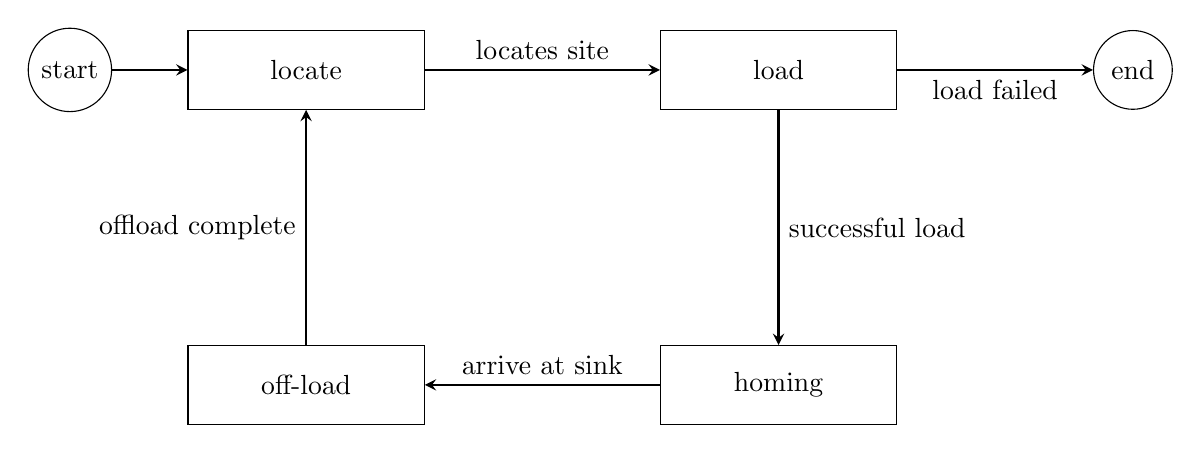
\begin{tikzpicture}[node distance=6cm]
	\node (locate) [process] {locate};
	\node[initial, left of=locate,xshift=3cm] (start) {start};
	\node (load) [process, right of=locate] {load};
	\node (homing) [process, below of=load,yshift=2cm] {homing};
	\node (offload) [process, left of=homing] {off-load};
	\draw [arrow] (locate) -- node[anchor=south] {locates site} (load);
	\node[initial, right of=load,xshift=-1.5cm] (end) {end};
	\draw [arrow] (load) -- node[anchor=west] {successful load} (homing);
	\draw [arrow] (homing) -- node[anchor=south] {arrive at sink} (offload);
	\draw [arrow] (offload) -- node[anchor=east] {offload complete} (locate);
	\draw [arrow] (start) -- node[anchor=east] {} (locate);
	\draw [arrow] (load) -- node[anchor=north] {load failed} (end);
	\end{tikzpicture}
	\caption{State Diagram of an Employed Forager Robot}
	\label{employedforagerstatediagram}
\end{figure}


The unemployed forager robot role allows the number of active robots in the environment to be regulated so that there are not too many robots attempting to forage or explore at once. An environment with too many employed foragers would result in more collisions between robots, which would mean that the employed foragers take longer to forage items. Also, if there are too many employed foragers in an environment which is sparse in items, then the employed foragers are not only causing collisions but they are also wasting energy by exploring areas unnecessarily.

Unemployed forager robots become scout robots if no scout robot broadcasts are detected for $t_{wait}$ time steps. The control parameter $t_{wait}$ is the maximum waiting time an unemployed forager can spend in the waiting state before switching to a scout robot, and $i_{wait}$ is the time spent by a robot in the waiting state. Decreasing $t_{wait}$ results in more scout robots exploring the environment and less unemployed foragers that a scout robot, who may have found quality sites, can recruit. Increasing $t_{wait}$ results in a greater number of unemployed forager robots waiting to be recruited. The greater number of unemployed foragers can form a large work force for a recruiting scout. However, too many unemployed foragers result in a smaller work force in the foraging environment.

\subsection{Initial States}
\label{initialstates}

A portion of the robots are initialized as scout robots in the explore state and the rest as unemployed forager robots. All robots are initialized adjacent to the sink. The percentage of robots initialized as scout robots is $X\in(0,100)$. Unemployed forager robots require a scout robot to recruit them to become employed forager robots. At initialization, the scout robots do not have site location details available, and therefore robots can not be initialized as employed forager robots. 

\subsection{Division of Labour}
\label{natureinspired:divisionoflabour}
The honey bee algorithm has two levels of division of labour. The first level is the division of labour between the scout, employed forager, and unemployed forager roles.

Another level of division of labour exists to deal with division of labour between foraging items with different priorities. Item-type division of labour is defined in this thesis as the division of labour between foraging prioritized item types and non-prioritized item types.

In nature, in times of drought, bees prioritize water over nectar or pollen. Honey bees would be sent out to forage for water but may encounter pollen while searching for water. If the foraging honey bee happens to encounter pollen, it will forage the pollen but will not communicate the discovery of the pollen site to the unemployed foragers \cite{seeley2009wisdom}. Using the bee's prioritization of resources as inspiration, the following rules for item-type division of labour are defined:

\begin{enumerate}
\item A scout robot that is set to search for the prioritized type (i.e. $\varsigma$ is set to prioritized items) will forage a non-prioritized type only if a prioritized item can not be located for the maximum time period, $f_{max}$. If $i_{explore} > f_{max}$ then $\varsigma$ will switch to foraging the non-prioritized type $\varsigma=\text{non-prioritized}$. The described rule is given explicitly in Algorithm~\ref{algorithm:explore}.
\item An employed robot foraging the non-prioritized item type will forage the non-prioritized item type until the robot fails to relocate a previously located non-prioritized item type site, or until the robot locates a prioritized item. For both of these cases, the robot will switch to foraging the prioritized item type $\varsigma=\text{non-prioritized}$.
\item A robot foraging a non-prioritized item will not communicate the location of the non-prioritized item site by dancing. 
\end{enumerate}

For the purposes of this study, each robot of each algorithm is assigned an initial item type to forage. The robots of the desert ant foraging algorithm and the na\"ive algorithm do not have item-type level division of labour and thus will continue to forage the same item-type that they were assigned throughout the experiment. The robots in the honey bee algorithm may switch what item-types they forage during the experiment, due to the item-type division of labour. 

\section{Methodology}
\label{methodology}


\subsection{Robots}
\label{chap:robots}

Foraging robots occur in all shapes, sizes and capabilities. Some robots have powerful GPS capabilities and advanced long distance sensors, while others are much simpler. This chapter defines the capabilities of the simulated robots to be used in this study. The robots are described in Section~\ref{robotdescription}, while Section~\ref{navigationandobstacleavoidance} outlines the navigational capabilities of the robots. 

\subsubsection{Robot Description}
\label{robotdescription}

The artificial robots modelled in this study are based on e-puck robots \cite{mondada2009puck}, with additional grippers. Each simulated robot is equipped with a 360 degree camera to identify objects around the robot, as well as eight local distance sensors equally spaced around the circular perimeter of the robot. Both camera and distance sensors have a depth of view of five times the robot's size. Robots use local communication which can occur in a radius of five times the robot's size. The sensor and communication range is sufficiently localized with respect to the size of the environment. Each simulated robot can forage a single item at a time. The robots do not have a global positioning system (GPS) capability to locate items to position themselves in the environment. A robot can not see occluded items. As a result, the simulated robots have to explore the environment to find the prioritized items.

%%%%%%%%%%%%%%%%%%%%%%%%%%%%%%%%%%%%%%%%%%%%%%%%%
%%%%%%%%%%%%%%%%%%%%%%%%%%%%%%%%%%%%%%%%%%%%%%%%%
\subsection{Simulator}
\label{simulator}
A spatially discrete 2-dimensional grid world simulator has been developed and used in this thesis in order to accelerate computation. Discrete 2-dimensional grid world simulators are also used in \cite{sugawara2002swarming, hecker2015beyond}. In real robot experiments, algorithm performance is sensitive to the amount of time taken to load items and manoeuvre the robots \cite{ostergaard2001emergent}. The 2-dimensional grid world simulator allows for movement and loading time to be standardized across all algorithms for effective comparison.

The simulated robots function as follows:
\begin{itemize}
	\item Each robot fits into one grid block and each item takes up one grid block. 
	\item Only a single object can occupy a grid block at a time.  An object is either a robot or an item. Since only one object can occupy a grid block at a time, collisions and congestion can occur.
	\item Each robot can move to an adjacent cell in any direction.
	\item Robots can load, transport and offload a single item at a time.
	\item If a robot cannot pick up an item, the item is an obstacle that a robot may have to navigate around in order to reach its destination.
\end{itemize}

The prioritized and non-prioritized sinks were placed next to each other, on a single side of the environment. The sinks were marked by beacons that all robots can detect and navigate towards. The reason why the sinks were not placed in the centre of the environment, as is commonly found in swarm robotics research \cite{labella2006division}, is because the prioritized foraging problem is inspired from using a swarm of robots to rescue trapped miners in mining tunnels, discussed in Section~\ref{sec:second:prioritizedforaging}. A mining tunnel has a single entrance where the gold and waste must be moved to, in order to be transported to the surface \cite{brune2010extracting}. Since there is only a single entrance at the beginning of a tunnel, the sinks need to occur at the beginning of the tunnel so that items can be easily exported.

\subsection{Environments}
\label{experimentenvironments}

In order to test flexiblity on different environment types, many types of environments should be examined. This section defines the various environments and presents how they were generated. Section~\ref{environmentalparameters} discusses the parameters for the environments, while different environment distributions, and the algorithms to generate those distributions are presented in Section~\ref{environmentdistributions}. Finally, the accessible environment is defined in Section~\ref{accessibleenvironment}.

\subsubsection{Environmental Parameters}
\label{environmentalparameters}
The experiments were run on different environments where each environment has different item distributions, environment sizes, item densities and different ratios of prioritized to non--prioritized items. All the environments are square. The length and width of the square environment grid is denoted as $\Lambda$, where $\Lambda\in \left\{ 50, 100, 200, 300, 500\right\}$.

Different values for the density, $p$, of the items on the grid were chosen, such that if $p=0.9$, then 90\% of the grid cells are occupied by items, where $p\in \{ 0.05,\allowbreak 0.2,\allowbreak 0.5,\allowbreak 0.7,\allowbreak 0.9\}$. Environments with a larger item density are more complex to forage, because there exists a higher probability that items will occlude each other. Thus, a robot may not be able to access items of the type that it is specialized to forage, since its access to those items is occluded by items of a different type. For this reason, we refer to the density of items on the grid as the problem complexity.

The environment type ratio, $r$, is defined as the ratio of prioritized to non-prioritized items in an environment, where $r\in \{0,\allowbreak 0.2,\allowbreak 0.25,\allowbreak 0.33,\allowbreak 0.5,\allowbreak 0.67,\allowbreak 0.75,\allowbreak 0.8, 1\}$. When $r=0$, an environment contains no prioritized items, and when $r=1$, only prioritized items exist in the environment. Environments with a small $r$ value have an abundance of non-prioritized items which increases the likelihood of non-prioritized items preventing access to prioritized items.

\subsubsection{Environment Distributions}
\label{environmentdistributions}
The environment distribution, $\epsilon$, is defined as the distribution of prioritized and non-prioritized items in an environment, such that $\epsilon\in\{uniform, clustered, gaussian, vein\}$. Each environment distribution was chosen in order to examine different characteristics of the algorithms. The item distributions are illustrated in Figure~\ref{fig:environments}, where each lighter shaded square is a prioritized item and a non-prioritized item is shown by a darker shaded square. The four environment distributions were generated as follows:

\begin{figure} [h]
        \centering
        \begin{subfigure}[b]{0.21\textwidth}
                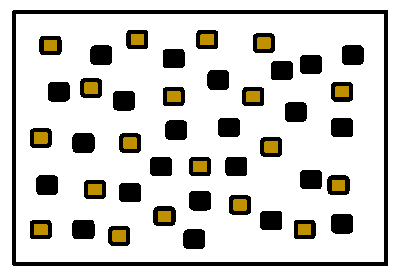
\includegraphics[width=\textwidth]{figures/uniformenv.pdf}
                \caption{Uniform}
                \label{fig:uniformenv}
        \end{subfigure}%
		\begin{subfigure}[b]{0.2\textwidth}
                        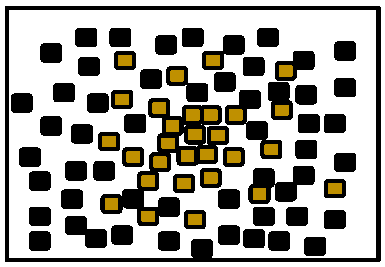
\includegraphics[width=\textwidth]{figures/gaussianenv}
                        \caption{Gaussian}
                        \label{fig:gaussianenv}
       \end{subfigure}
        \begin{subfigure}[b]{0.205\textwidth}
                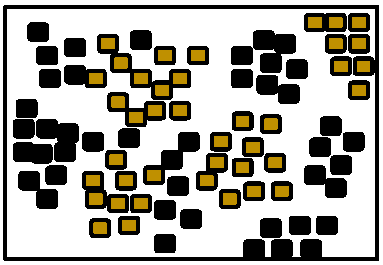
\includegraphics[width=\textwidth]{figures/clusterenv.pdf}
                \caption{Clustered}
                \label{fig:clusterenv}
        \end{subfigure}
        \begin{subfigure}[b]{0.2\textwidth}
                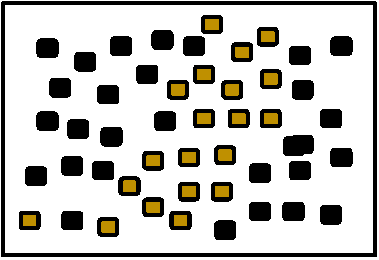
\includegraphics[width=\textwidth]{figures/veinenv.pdf}
                \caption{Vein}
                \label{fig:veinenv}
        \end{subfigure}  

		\caption{Environment Classes}
		\label{fig:environments}
\end{figure}

\begin{algorithm}

\caption{Uniform Distributed Environments}
\label{algorithm:uniform}
\begin{algorithmic}[1]
\Function{uniform}{$numberItems, r, S$}
	\State \text{nonPrioritizedItemsLeft = floor((1-$r$)*numberItems)}
	\State \text{prioritizedItemsLeft = floor( $r$*numberItems)}
	\While{\text{$prioritizedItemsLeft > 0$}}
		\State \text{x $\gets$ uniform(0, S)}
		\State \text{y $\gets$ uniform(0, S)}
		\If{\text{gridCell (x,y) is empty}}
			\State \text{Place prioritized item at (x,y)}
			\State \text{Decrement $prioritizedItemsLeft$}
		\EndIf
	\EndWhile

	\While{\text{$nonPrioritizedItemsLeft > 0$}}
		\State \text{x $\gets$ uniform(0, S)}
		\State \text{y $\gets$ uniform(0, S)}
		\If{\text{gridCell (x,y) is empty}}
			\State \text{Place prioritized item at (x,y)}
			\State \text{Decrement $nonPrioritizedItemsLeft$}
		\EndIf
	\EndWhile
\EndFunction
\end{algorithmic}
\end{algorithm}

\begin{enumerate}

\item The position of each item in a uniformly distributed environment is selected from a uniform distribution (refer to Figure~\ref{fig:uniformenv}). The uniformly distributed environment has uniform concentrations of prioritized and non-prioritized items across the environment and thus is used as a control environment. Pseudo-code for generation of uniform environments is provided in Algorithm~\ref{algorithm:uniform}.

\item For the Gaussian environments, the positions of the prioritized items are sampled from a Gaussian distribution. The mean of the Gaussian disitribution is the centre of the grid. The deviation of the Gaussian distribution was selected as $deviation = S*E_p/2$ to ensure that generation took a reasonable amount of time (that the same positions are not reselected regularly), and that the non-prioritized items are densely concentrated  (refer to Figure~\ref{fig:gaussianenv}). Pseudo-code for generation of Gaussian environments is provided in Algorithm~\ref{algorithm:gaussian}. The positions of the non-prioritized items are selected from a uniform distribution, after placing the prioritized items. 

In Gaussian distributed environments, prioritized items  occur in high concentration towards the center of the environment. More non-prioritized items occur on the outskirts of the environment, surrounding the prioritized items in the centre.

The Gaussian environments are used to examine whether each algorithm will enable the robot swarm to forage or navigate past the non-prioritized items to reach the high concentration of prioritized items in the environment's centre. 


\item Environments with a vein distribution resemble the patterns observed in naturally occurring gold reefs \cite{frimmel2002recent} (refer to Figure~\ref{fig:veinenv}). In a gold reef, molten gold fills planar fractures between rock resulting in a vein of gold. Inspired by gold reefs, vein distributed environments have a long thin vein of prioritized items running from one side of the environment to another. The vein of prioritized items was surrounded by non-prioritized items. 

The vein environments aimed to test whether a swarm of robots could forage the continuous length of the vein of prioritized items, before foraging non-prioritized items. A swarm that is able to detect the location of the vein and return to the vein's location after foraging an item should forage more prioritized items initially than an algorithm that cannot detect and remember the location of the vein.  Pseudo-code for generation of vein environments is provided in Algorithm~\ref{algorithm:vein}.


\item Environments with a clustered item distribution have a random number of clusters of items of the same type (refer to Figure~\ref{fig:clusterenv}). After clusters have been generated, each cluster is labelled randomly (with a Bernoulli disitribution with probability equal to the item ratio, $r$, required for that environment), as either a cluster of prioritized items or a cluster of non-prioritized items.

The goal of performing experiments in a clustered environment was to test an algorithm's ability to exploit areas which are rich in prioritized items. Clustered environments are also used to test whether an algorithm can either navigate around or forage non-prioritized items. A clustered environment can also test an algorithm's ability to remember locations of areas which have a high density of prioritized items in order to aid more efficient access to prioritized items.  Pseudo-code for generation of clustered environments is provided in Algorithm~\ref{algorithm:clustered} and Algorithm~\ref{algorithm:clustered2}.


\end{enumerate} 

To summarize, the challenges introduced by the more complex distributions (the Gaussian, clustered and vein environment) aim to test a swarm's ability to:

\begin{itemize}
\item navigate past obstacles efficiently, or alternatively, to forage obstacles efficiently, and to
\item return to areas rich in prioritized items to forage these areas.
\end{itemize}



\begin{algorithm}
\caption{Gaussian Distributed Environments}
\label{algorithm:gaussian}
\begin{algorithmic}[1]
\Function{gaussian}{$numberItems, r, S$}
	\State \text{Calculate environment centre point $(x_c, y_c)$}
	\State \text{prioritizedItemsLeft = floor($r$*numberItems)}
	\State \text{nonPrioritizedItemsLeft = floor((1-$r$)*numberItems)}
	\State \text{deviation = S*$r$/2}
	\While{\text{$prioritizedItemsLeft > 0$}}
		\State \text{$x \gets floor(gaussian(x_c, deviation))$}
		\State \text{$y \gets floor(gaussian(y_c, deviation))$}
		\If{\text{gridCell (x,y) is empty and is valid}}
			\State \text{Place prioritized item at (x,y)}
			\State \text{Decrement $prioritizedItemsLeft$}
		\EndIf
	\EndWhile

	\While{\text{$nonPrioritizedItemsLeft > 0$}}
		\State \text{x $\gets$ uniform(0, S)}
		\State \text{y $\gets$ uniform(0, S)}
		\If{\text{gridCell (x,y) is empty}}
			\State \text{Place non prioritized item at (x,y)}
			\State \text{Decrement $nonPrioritizedItemsLeft$}
		\EndIf
	\EndWhile
\EndFunction
\end{algorithmic}
\end{algorithm}


\begin{algorithm}
\caption{Vein Distributed Environments}
\label{algorithm:vein}
\begin{algorithmic}[1]
\Function{vein}{$numberItems, r, S$}
	\State \text{Select two random sides from the grid}
	\State \text{Select a random points on each sides, $(x_0,y_0)$ and $(x_1,y_1)$}
	\State \text{Calculate gradient of vein, $m = (y_0 - y_1)/(x_0 - x_1)$}
	\State \text{Calculate $c$ of equation for line vein, $c = (y_0 - m*x_0)$
}

	\State \text{prioritizedItemsLeft = floor($r$*numberItems)}
	\State \text{nonPrioritizedItemsLeft = floor((1-$r$)*numberItems)}

	\While{\text{$prioritizedItemsLeft > 0$}}
		\State \text{$x \gets uniform(min(x_0,x_1), max(x_0, x_1))$}
		\State \text{$y \gets m*x + c$}
		\If{\text{gridCell (x,y) is valid and gridCell (x,y) is empty}}
			\State \text{Place prioritized item at (x,y)}
			\State \text{Decrement $prioritizedItemsLeft$}
		\EndIf
	\EndWhile

	\While{\text{$nonPrioritizedItemsLeft > 0$}}
		\State \text{x $\gets$ uniform(0, S)}
		\State \text{y $\gets$ uniform(0, S)}
		\If{\text{gridCell (x,y) is empty}}
			\State \text{Place nonprioritized item at (x,y)}
			\State \text{Decrement $nonPrioritizedItemsLeft$}
		\EndIf
	\EndWhile
\EndFunction
\end{algorithmic}
\end{algorithm}


\begin{algorithm}

%TODO
\caption{Clustered Distributed Environments (Part 1)}
\label{algorithm:clustered}
\begin{algorithmic}[1]
\Function{clustered}{$numitems, r, S$}
  \State \text{Generate number of clusters, $total = uniform(3,15)$}
  \State \text{Calculate number of prioritized clusters, $clusters_p = floor(r*total)$}    
  \State \text{Calculate number of non-prioritized clusters, $clusters_{np} = floor((1-r)*total)$}
  
  \State \text{Calculate number of prioritized items, $total_p = floor(r*numitems)$}
  
  \State \text{Calculate number of non-prioritized items, $total_{np} = floor((1-r)*numitems)$}
  
  \State \text{$ave_p = total_p/clusters_{p}$}
  \State \text{$ave_np = total_{np}/clusters_{np}$}
  \State \text{$clustersToGenerate_p = clusters_p$}
  \State \text{$clustersToGenerate_{np} = clusters_{np}$}

  \While{\text{$clustersToGenerate_p > 0$}}
    \State \text{sample centroid for cluster $C$ (x,y) uniformly from grid}
    \State \text{$num_p = uniform(ave_p/2$, $2*ave_p$)}
    \State \text{Calculus radius, $r$, of cluster $C$ as $r = \sqrt{num_p/\pi}$}
    \If{\text{cluster $C$ does not collide with existing clusters}}
      \State \text{Save centroid and radius of cluster $C$ to list}
      \State \text{Decrement $clustersToGenerate_p$}
      \State \text{$itemsToGenerate_p = num_p$}
          
      \While {$itemsToGenerate_p > 0$}
        \State \text{$x_p = gaussian(x, r)$}
        \State \text{$y_p = gaussian(y, r)$}
        \If{\text{position $(x_{p},y_{p})$ is valid}}
          \State \text{Place prioritized item at $(x_p,y_p)$}
          \State \text{Decrement $itemsToGenerate_{np}$}	
        \EndIf
      \EndWhile
    \EndIf
  \EndWhile
  \algstore{clusteredalg}
\end{algorithmic}
\end{algorithm}
  
\begin{algorithm}

%TODO
\caption{Clustered Distributed Environments (Part 2)}
\label{algorithm:clustered2}
\begin{algorithmic}[1]
  \algrestore{clusteredalg}
  \While{\text{$clustersToGenerate_{np} > 0$}}
	  \State \text{sample centroid for cluster $C$ (x,y) uniformly from grid}
	  \State \text{$num_{np}=uniform(ave_{np}/2,2ave_{np})$}
	  \State \text{Calculus radius, $r$, of cluster $C$ as $r = \sqrt{num_{np}/\pi}$}
	  \If{\text{cluster $C$ does not collide with existing clusters}}
	
		  \State \text{Save centroid and radius of cluster $C$ to list}
		  \State \text{Decrement $clustersToGenerate_{np}$}
		  \State \text{$itemsToGenerate_{np} = num_{np}$}
				
		  \While {$itemsToGenerate_{np} > 0$}
        	\State \text{$x_p = gaussian(x, deviation=r)$}
        	\State \text{$y_p = gaussian(y, deviation=r)$}
			\If{\text{position $(x_{np},y_{np})$ is valid}}
				  \State \text{Place non-prioritized item at $(x_{np},y_{np})$}
				  \State \text{Decrement $itemsToGenerate_{np}$}	
			  \EndIf
		  \EndWhile
		\EndIf
	\EndWhile
\EndFunction
\end{algorithmic}
\end{algorithm}


\subsubsection{Accessible Environment}
\label{accessibleenvironment}

To aid discussions about the algorithms' performance on different types of environments, the concept of an \textbf{accessible environment} should be introduced. For the purposes of this thesis, an accessible environment is the parts of the environment that can be foraged by the swarm and are not blocked by other items. Items that are hidden behind other items are not accessible to the robot swarm and are thus not part of the accessible environment. The accessible environment is much larger in a less densely populated environment. This also introduces the concept of the environment ratio of a given accessible environment. For example, an environment may have a high ratio of prioritized items overall, but if the prioritized items are surrounded completely by non-prioritized items, then the accessible environment consists only of non-prioritized items and has an environmental item type ratio of 0. The environment ratio of the accessible environment changes differently per environment disitribution type. In high density Gaussian environments, the accessible environment will initially consist of mostly non-prioritized items, but as robots forage towards the centre, the accessible environment will consist largely of prioritized items. For uniform environments, all accessible environments would have a similar or same environment item ratio as the entire environment. In clustered environments, depending on the configuration of the clusters, the environment ratio of the accessible environments would vary. For vein environments, at the beginning of foraging, the accessible environment ratio would be low in high density environments if the vein is perpendicular to the sink since only the ``entrance" of the prioritized vein would be exposed to the robots and the rest of the prioritized items would be stacked behind those items. 

\subsection{Swarm parameters}
\label{swarmparameters}

For all algorithms, each robot swarm was initialized with a swarm specialization ratio, $\tau\in\left\{0, 0.2, 0.25, 0.333, 0.5, 0.667, 0.75, 0.8,1\right\}$. The swarm specialization ratio is the ratio of robots foraging prioritized items to non-prioritized items. When no robots are set to initially forage prioritized items, then $\tau=0$ and when all robots are set to initially forage prioritized items, then $\tau=1$.

The ability of an algorithm to adapt the value of $\tau$ appropriately for a given $r$ indicates the flexibility of the algorithm.

The swarm density, $c$, is defined as the number of cells occupied by a robot, as a percentage of the grid size $\Lambda$ (the length of the side of an environment), where values of $c\in\left\{0.1, 0.3, 0.5, 0.7, 1\right\}$ were evaluated. The swarm density is varied in order to test the scalability of the algorithm. The swarm density is also varied to test each algorithms' ability to adjust the number of actively foraging robots to the density of the items in the environment, $c$, as well as to adjust the number of robots actively foraging an item type, $\tau$, to the item type density, $r$.

The honey bee algorithm specific parameters were selected based on \cite{seeley2009wisdom}, where $t_{wait}=200$ time steps, $f_{max}=100$ time steps, $\Phi=0.8$ and $\rho=0.1$. Testing the effect of each of the parameters specific to the honey bee algorithm was not in the scope of this thesis.

\subsection{Experimentation}
\label{experimentation}

The initial position of each robot was randomly selected, adjacent to the sink. For the na\"ive algorithm and desert ant algorithm, all robots began in the exploration state. For the honey bee algorithm, all unemployed foraging robots were initialized in the waiting state, and the scout robots were initialized in the explore state. 
An experiment is defined as the 30 independant runs for each algorithm, with a specific set of swarm parameters, and on an environment which has a specific set of environmental parameters. An experiment is run for every possible combination of swarm and environmental parameters.

\subsection{Performance measures}
\label{thri:third:performancemeasures}

The performance of swarm robotics algorithms can be measured by examining the algorithm's ability to perform a task in terms of efficiency, scalability, flexibility, and robustness.

\subsection{Foraging Efficiency}
\label{setup:foragingefficiency}
The foraging efficiency, $E_P$, of an algorithm is defined as the ratio of the number of prioritized items collected by all robots in a fixed time period on a specific environment to the total number of prioritized items that exist in the environment. The foraging efficiency metric is similar to the efficiency metric used by Hecker \textit{et al} \cite{hecker2015beyond}. The metrics used in experiments performed by Hecker \textit{et al} evaluate the performance of foraging algorithms and are thus appropriate for use in the experiments of this study. The foraging efficiency measure, $E_P$, only considers the prioritized items for the prioritized foraging problem.


\subsubsection{Flexibility}
\label{setup:flexibility}

As stated in Section~\ref{flexibility}, flexibility refers to the effect of variations in the environment and tasks on the co-ordination mechanisms of swarm robotics algorithms. An algorithm that is highly flexible is one that has been optimized for a specific environment, but is equally efficient on a different environment \cite{hecker2015beyond}.

The flexibility performance measures used in this study are based on the flexibility performance measures used in \cite{hecker2015beyond}, which have been adapted for the prioritized foraging problem by only taking into account the prioritized item. The flexibility study addresses two aspects: Flexibility with respect to different prioritized item ratios, $r$, and flexibility with respect to different environment distributions.

In order to more succinctly define the flexibility performance measures, the following notation is defined:

Let $\overline{r}$ be the list containing all considered elements for environment item type ratio, $r$, and let $n_r$ be the number of elements in the list. Let $\overline{\tau}$ be the list containing all considered elements for initial swarm specialization ratio, $\tau(0)$, and let the number of elements in the list be $n_t$. Similarly, let $\overline{\epsilon}$ be a list of each environment distribution and let $n_\epsilon$ be the number of elements in the list.

Let $Z$ be a matrix of dimensions $n_t \times n_r$. Define each entry of the matrix $Z_{ij}$ as the average foraging efficiency, $E_P$, over all experiments, for a specific environment ratio $r_j$, where $r_j$ is the $j$th element of $\overline{r}$, and for a specific initial swarm specialization ratio $\tau_i(0)$, such that $\tau_i(0)$ is the $i$th element of $\overline{\tau}$.

Similarly, define matrix $D$ with dimensions $n_t \times n_\epsilon$, such that each entry of the matrix $D_{ij}$ is the average foraging efficiency, over all experiments with environment distribution, $\epsilon_j$, and with the initial swarm initialization ratio, $\tau_i(0)$.


%\subsubsection{Flexibility with respect to different prioritized item ratios}
%\label{setup:flexibility:prioritizeditemratio}

The goal of examining flexibility over different prioritized item ratios is to determine how well the optimum value for initial swarm specialization ratio, $\tau(0)$, for a specific environment item ratio, $r_u$, generalizes across all other environment item ratios, $r_v$, where $u,v = 1,...,n_r$ and $u \neq v$. The optimum value for $\tau(0)$ for environments of a specific environment item ratio is the value that yields the greatest average efficiency for those environments.

To do so, a list $I$ of size $n_r$ is defined, where each entry $I_j$ is set to the index $k$ that yields the maximum value for $Z_{ij}$, for $i = 1,..., n_\tau$, for environments with a specific environment type ratio $r_j$. More succinctly:

\begin{equation}
I_j = ( k | Z_{kj} = \max_{i=1,...,n_\tau}\{Z_{ij}\} )
\end{equation}

The moment, $F_{r_u}$, around the maximum foraging efficiency for a specific environment item type ratio, $r_u$, is defined as follows: 

\begin{equation}
F_{r_u} = \sum_{v=1}^{n_r}\dfrac{|Z_{I_uu}- Z_{I_uv}|}{Z_{I_uu}}
\end{equation}

The final performance measure is the normalized sum of the above moments around the maximum foraging efficiency for every environment item type ratio in $\overline{r}$:

\begin{equation}
F_r = \dfrac{1}{n_r}\sum_{u=1}^{n_r} F_{r_u}
\end{equation}

The performance measure, $F_r$, measures how well swarm parameters, which are optimized to yield the best efficiency for environments with a specific prioritized item ratio generalize across environments with different prioritized item ratios. The less the foraging efficiency varies when an algorithm that is configured with swarm parameters optimized for a specific environment ratio, is run on all other environment ratios, the smaller $F_r$ will be. Therefore, the smaller $F_r$ is, the more flexible an algorithm is considered to be. $F_r$ is a macro performance indicator which is run on the results of all experiments. 


%\subsubsection{Flexibility with respect to different environment distributions}
%\label{setup:flexibility:environmentdistributions}


This performance measure evaluates flexibility by analysing how well swarm parameters, which are optimized to yield the best efficiency for environments with a specific environment distribution generalize across environments with different environment distributions. The performance measure, $F_{\epsilon}$, is defined similar to $F_r$, except over environment distributions, rather than environmental item ratios. A list $Y$ of size $n_\epsilon$ is defined as follows:

\begin{equation}
Y_j = ( k | D_{kj} = \max_{i=1,...,n_\tau}\{D_{ij}\} )
\end{equation}

The performance measure, $F_\epsilon$, is defined as follows:

\begin{equation}
F_\epsilon = \dfrac{1}{n_\epsilon}\sum_{u=1}^{n_\epsilon} \sum_{v=1}^{n_\epsilon}\dfrac{|D_{Y_uu}- D_{Y_uv}|}{D_{Y_uu}}
\end{equation}

$F_\epsilon$ is interpreted in a similar manner to $F_r$, where the smaller the value for $F_\epsilon$ is, the more flexible an algorithm is considered to be over environment distributions.

\subsubsection{Scalability}
\label{setup:scalability}

Scalability is described in Section~\ref{sr:scalabilty}. The scalability performance measures used in this thesis are based on the measures used in \cite{hecker2015beyond}. This study analyses the scalability of each of the algorithms with respect to two performance measures, namely, swarm density scalability and problem complexity scalability. Swarm density scalability and problem complexity scalability are defined in the following sections. Both swarm density scalability and problem complexity scalability are evaluated on the largest environment size (i.e. $\Lambda=500$) in order to prevent the possibility that an environment runs out of items to forage.

To simplify the explanation of the scalability performance measures, the following notation is defined:

Let $\overline{c}$ be the list of all considered values for swarm density, $c$, with length $n_c$. Let $c_{min}$ be the minimum value considered for $c$ and $c_i$ be the $i$th value of $\overline{c}$. Let $E_{c_i}$ be the average foraging efficiency, $E_P$, over all experiments, with swarm density $c_i$.

Similarly, define the list of all considered values for problem complexity, $p$, as $\overline{p}$ with length $n_p$. The smallest problem complexity is $p_{min}$ and $E_{p_i}$ is the average foraging efficiency over all experiments, with problem complexity $p_i$.


%\subsubsection{Swarm density scalability}
%\label{swarmsizescalability}

The efficiency of a robot swarm should be relatively undisturbed by changes in group sizes. This property is known as swarm density scalability. Ideally, foraging efficiency should increase linearly as swarm density increases, which is known as linear scalability. However, due to increased inter-robot interference in larger swarm densities, scalability is often sub-linear (i.e. logarithmic) \cite{lerman2002mathematical}. Many swarm robotics algorithms focus on the use of division of labour, navigation or communication in order to decrease inter-robot interference \cite{lerman2002mathematical, schneider1998territorial}.

In order to analyse swarm scalability, one could simply examine the average efficiency of each algorithm, over all experiments, at each swarm density. However, to ensure that each algorithm is compared on scalability alone, the individual efficiencies of each algorithm must be eliminated. To eliminate the individual efficiencies of each algorithm, the average efficiency, $E_{c_i}$, for each swarm density, $c_i$, is normalized by the average efficiency, , $E_{c_{min}}$, for the smallest sized swarm for that algorithm, as follows: 

\begin{equation}
S_{c_i} = \dfrac{E_{c_{i}} - E_{c_{min}}}{E_{c_{min}}}
\end{equation}


To analyse how each algorithm scales, the normalized average foraging efficiency, $S_{c_i}$, for each value in $\overline{c}$ can be plotted for each algorithm to determine whether an algorithm scales linearly, sublinearly, or superlinearly. 

The total swarm scalability, $S_c$, provides a single value per algorithm, which can be used to compare overall swarm scalability:

\begin{equation}
	S_c = \sum_{i=1}^{n_c} S_{c_i}
\end{equation}


The larger the value of $S_c$, the better foraging efficiency scales with respect to swarm density. 


%\subsubsection{Problem complexity scalability}
%\label{setup:problemscalability}

Ideally, foraging efficiency should be indirectly proportional to problem complexity. As the problem complexity increases, the foraging efficiency should decrease linearly. An algorithm is scalable when performance decreases linearly or sublinearly as efficiency increases. Similar to swarm density scalability (described in Section~\ref{swarmsizescalability}) problem complexity scalability is often sub-linear, due to increased environmental interference. 

In order to evaluate the problem scalability of each of the algorithms presented, the efficiency of each algorithm is examined over a variety of environment item densities, $p$, defined in Section~\ref{experimentenvironments}. Similar to swarm density scalability performance measures $S_{c_i}$ and $S_c$, the problem complexity scalability measures, $S_{p_i}$ and $S_p$, are defined as follows:

\begin{equation}
	S_{p_i} = \dfrac{E_{p_{i}} - E_{p_{min}}}{E_{p_{min}}}
\end{equation}

\begin{equation}
	S_p = \sum_{i=1}^{n_p} S_{p_i}
\end{equation}

\subsubsection{Behavioural Performance Measures}
\label{behaviouralperformancemeasures}

Despite not being one of the more typical performance measures for swarm robotics, a number of measures are included to enable further understanding of the obtained quantitive performance measures.

\subsubsection{Items foraged over time}
To give insight into the effects of environmental and swarm parameters on overall performance, and to characterise the effects of certain behaviours, the following metrics have been recorded:

\begin{itemize}
\item The total number of prioritized items foraged over time, $E^t_P$. The total number of prioritized items foraged are recorded every 200 time steps and are normalized with the total number of prioritized items that exists in the specific environment.
\item The total number of non-prioritized items foraged over time, $E^t_{NP}$. The total number of non-prioritized items foraged are recorded every 200 time steps and are normalized with the total number of non-prioritized items that exist in the specific environment.
\end{itemize}

\subsubsection{Swarm specialization ratio over time}
Swarm specialization ratio stays constant for the desert ant algorithm and the na\"ive algorithm, but the swarm specialization ratio changes for the honey bee algorithm, due to the division of labour mechanisms. In order to gain a better understanding of how the division of labour mechanism performs, the swarm specialization ratio over time, $\tau(t)$, is tracked. The swarm specialization ratio is recorded every 200 time steps.

\subsubsection{Time spent performing recruitment}
Unlike the desert ant algorithm and the na\"ive algorithm, the honey bee algorithm robots perform behaviours that are not directly involved in retrieving items - in particular, the recruitment activities form part of the division of labour mechanism. In order to better understand the influence of the division of labour mechanisms, the average percentage of the time that each robot spents on each division of labour activity is recorded as follows:

\begin{itemize}
\item $t_{wait}$, the average percentage of the total number of time steps spent by each robot in the waiting state.
\item $t_{recruitment}$, the average percentage of the total time number of steps spent by each robot in the recruitment state.
\end{itemize}


\section{Results}
\label{results}

The analysis of the results of the experiments is organised with respect to four major characteristics of swarm robotics algorithms, namely efficiency, flexibility, robustness, and scalability. Section~\ref{results:efficiency} addresses foraging, while the flexibility of the algorithms over different environment distributions and item type ratios is analysed in Section~\ref{results:flexibility}. Section~\ref{results:scalability} evaluates the scalability of each algorithm, and robustness is analysed in Section~\ref{results:robustness}. Section~\ref{results:summary} summarizes the findings of the analysis.

\subsection{Foraging efficiency}
\label{results:efficiency}


Despite the fact that determining the most efficient algorithm is not a main focus of this study, this section does a brief comparison of the foraging efficiency, $E_P$ (defined in Section~\ref{setup:foragingefficiency}), of each algorithm. 

This is done by comparing the performance of the three algorithms over all environments and all swarm parameters giving a total at 121500 unique experiment configurations each run for 30 independant samples. A Wilcoxin test, at a confidence level of 0.05, was applied over the 30 independant samples, for each pair of algorithms, for each experiment, to determine if a statistically significant difference in foraging efficiency of the pair of algorithms exists. If no statistically significant difference is indicated between the two algorithm experiment samples, then nothing is done. If a statistically significant difference is indicated between the two algorithm experiment samples, then two one-tailed Mann-Whitney U tests were performed at a significance level of 0.05 to determine which algorithm had a greater foraging efficiency on a particular experiment. Suppose $A$ and $B$ are two of the selected algorithms. If the first one-tailed Mann-Whitney U test indicates that $A$ is significantly more efficient than $B$, then a ``win" is counted for algorithm $A$. If the second one-tailed Mann-Whitney U test indicates that the $E_P$ for $A$ is significantly less efficient than $B$, then a ``loss" is counted for algorithm $A$. 

To determine an algorithm's foraging efficiency in comparison to each other algorithm, the wins and losses for each algorithm are summed per experiment. This statistical analysis approach has been used in \cite{helbig2013performance}. The percentage of wins per algorithm and the percentage of losses per algorithm is calculated, because percentages are more informative than counts. The percentage of wins per algorithm and the percentage of losses per algorithm are summarized in Table~\ref{summarytable}. The desert ant foraging performed better than the na\"ive algorithm. The honey bee algorithm out-performed both the na\"ive algorithm and the desert ant algorithm. The following sections analyse the swarm robot properties of each algorithm, and explain why the foraging efficiency of the algorithms is as shown in Table~\ref{summarytable}.


\begin{table}[!htbp]
    \centering
    \caption{Pairwise one-tailed Mann Whitney U wins and loss counts, for the foraging efficiency, $E_P$, for each algorithm, over all environments and swarm parameter values }
    \label{summarytable}
    \begin{tabular}{@{}lll@{}}
    \toprule
    \textbf{Algorithms} & \textbf{Wins} & \textbf{Losses} \\ \midrule
    Na\"ive               & $1.3\%$          & $66.5\%$           \\
    Desert ant          & $47.4\%$         & $16.4\%$           \\
    Honey bee           & $51.2\%$         & $17.1\%$          \\ \bottomrule
    \end{tabular}
\end{table}


\subsection{Flexibility}
\label{results:flexibility}

This section analyses the flexibility of each of the considered algorthms in terms of the prioritized item ratio and the environment distribution types, over all experiments. Section~\ref{results:prioritizeditemratio} analyses the flexibility of each algorithm in terms of the prioritized item ratio of the environment. Section~\ref{results:flexibility:environmentdistribution} discusses the flexibility of each algorithm in terms of environment distribution types.
\subsubsection{Flexibility in terms of prioritized item ratio}
\label{results:prioritizeditemratio}

The performance measure, $F_r$ (defined in Section~\ref{setup:flexibility:prioritizeditemratio}), measures how well the swarm parameters, which yield the best efficiency for environments with a specific prioritized item ratio, generalize across environments with different prioritized item ratios. Therefore, the smaller $F_r$ is, the more flexible an algorithm is considered to be. $F$ is a macro performance indicator which is run on the results of all experiments. 

Table~\ref{table:flexibility} summarizes the flexibility of each foraging algorithm in terms of environment type ratio, $F_r$. According to Table~\ref{table:flexibility}, the honey bee algorithm is the most flexible in terms of $F_r$, followed by the na\"ive algorithm, with the desert ant algorithm exhibiting the worst flexibility. 

 
% Please add the following required packages to your document preamble:
% \usepackage{booktabs}
\begin{table}[!htbp]
\centering
\caption{Flexibility in terms of prioritized item ratio, $F_r$, and flexibility in terms of environment distribution, $F_\epsilon$, for each algorithm}
\label{table:flexibility}
\begin{tabular}{@{}llll@{}}
\toprule
\textbf{}         & Na\"ive         & Desert ant        & Honey bee         \\ \midrule
\textbf{$F_r$}    & 1.186 & 3.124     & 0.828    \\ \midrule
\textbf{$F_\epsilon$} & 1.112 & 0.507 & 0.458 
\end{tabular}
\end{table}

The honey bee algorithm is the most flexible in terms of prioritized item ratio. To understand why this is the case, the mechanisms used specifically by the honey bee algorithm have to be examined. In particular, the honey bee algorithm employs a division of labour mechanism that allows robots to switch from foraging prioritized items to non-prioritized items (and vice versa). The honey bee algorithm's division of labour mechanism suggests the following hypothesis: The honey bee algorithm's superior flexibility is due to the fact that the robots can switch their item type specialization. In that way, the honey bee algorithm was able to adapt the swarm specialization ratio to more efficiently forage a given environment item type ratio.

To provide evidence for the above hypothesis the average swarm specialization ratio over time, $\tau(t)$, for the honey bee algorithm on a uniformly distributed environment with a high ratio of prioritized items (i.e. $r = 0.75$) is examined. The initial swarm specialization ratio, $\tau(0)$, was set to 0, which means that all robots are set to forage non-prioritized items. The swarm specialization ratio over time, $\tau(t)$, was averaged over 30 independant runs. The purpose behind examining the described scenario is to determine if the honey bee algorithm is able to adapt the swarm's specialization ratio (which initially can only forage non-prioritized items), to more efficiently forage the high ratio of prioritized items. The above scenario is illustrated in Figure~\ref{fig:specializationratioovertime}. 


\begin{figure}[!htb]
\centering
\resizebox{\textwidth}{!}{% GNUPLOT: LaTeX picture with Postscript
\begingroup
  \makeatletter
  \providecommand\color[2][]{%
    \GenericError{(gnuplot) \space\space\space\@spaces}{%
      Package color not loaded in conjunction with
      terminal option `colourtext'%
    }{See the gnuplot documentation for explanation.%
    }{Either use 'blacktext' in gnuplot or load the package
      color.sty in LaTeX.}%
    \renewcommand\color[2][]{}%
  }%
  \providecommand\includegraphics[2][]{%
    \GenericError{(gnuplot) \space\space\space\@spaces}{%
      Package graphicx or graphics not loaded%
    }{See the gnuplot documentation for explanation.%
    }{The gnuplot epslatex terminal needs graphicx.sty or graphics.sty.}%
    \renewcommand\includegraphics[2][]{}%
  }%
  \providecommand\rotatebox[2]{#2}%
  \@ifundefined{ifGPcolor}{%
    \newif\ifGPcolor
    \GPcolorfalse
  }{}%
  \@ifundefined{ifGPblacktext}{%
    \newif\ifGPblacktext
    \GPblacktexttrue
  }{}%
  % define a \g@addto@macro without @ in the name:
  \let\gplgaddtomacro\g@addto@macro
  % define empty templates for all commands taking text:
  \gdef\gplbacktext{}%
  \gdef\gplfronttext{}%
  \makeatother
  \ifGPblacktext
    % no textcolor at all
    \def\colorrgb#1{}%
    \def\colorgray#1{}%
  \else
    % gray or color?
    \ifGPcolor
      \def\colorrgb#1{\color[rgb]{#1}}%
      \def\colorgray#1{\color[gray]{#1}}%
      \expandafter\def\csname LTw\endcsname{\color{white}}%
      \expandafter\def\csname LTb\endcsname{\color{black}}%
      \expandafter\def\csname LTa\endcsname{\color{black}}%
      \expandafter\def\csname LT0\endcsname{\color[rgb]{1,0,0}}%
      \expandafter\def\csname LT1\endcsname{\color[rgb]{0,1,0}}%
      \expandafter\def\csname LT2\endcsname{\color[rgb]{0,0,1}}%
      \expandafter\def\csname LT3\endcsname{\color[rgb]{1,0,1}}%
      \expandafter\def\csname LT4\endcsname{\color[rgb]{0,1,1}}%
      \expandafter\def\csname LT5\endcsname{\color[rgb]{1,1,0}}%
      \expandafter\def\csname LT6\endcsname{\color[rgb]{0,0,0}}%
      \expandafter\def\csname LT7\endcsname{\color[rgb]{1,0.3,0}}%
      \expandafter\def\csname LT8\endcsname{\color[rgb]{0.5,0.5,0.5}}%
    \else
      % gray
      \def\colorrgb#1{\color{black}}%
      \def\colorgray#1{\color[gray]{#1}}%
      \expandafter\def\csname LTw\endcsname{\color{white}}%
      \expandafter\def\csname LTb\endcsname{\color{black}}%
      \expandafter\def\csname LTa\endcsname{\color{black}}%
      \expandafter\def\csname LT0\endcsname{\color{black}}%
      \expandafter\def\csname LT1\endcsname{\color{black}}%
      \expandafter\def\csname LT2\endcsname{\color{black}}%
      \expandafter\def\csname LT3\endcsname{\color{black}}%
      \expandafter\def\csname LT4\endcsname{\color{black}}%
      \expandafter\def\csname LT5\endcsname{\color{black}}%
      \expandafter\def\csname LT6\endcsname{\color{black}}%
      \expandafter\def\csname LT7\endcsname{\color{black}}%
      \expandafter\def\csname LT8\endcsname{\color{black}}%
    \fi
  \fi
    \setlength{\unitlength}{0.0500bp}%
    \ifx\gptboxheight\undefined%
      \newlength{\gptboxheight}%
      \newlength{\gptboxwidth}%
      \newsavebox{\gptboxtext}%
    \fi%
    \setlength{\fboxrule}{0.5pt}%
    \setlength{\fboxsep}{1pt}%
\begin{picture}(7200.00,5040.00)%
    \gplgaddtomacro\gplbacktext{%
      \csname LTb\endcsname%
      \put(740,640){\makebox(0,0)[r]{\strut{}$0$}}%
      \put(740,1056){\makebox(0,0)[r]{\strut{}$0.1$}}%
      \put(740,1472){\makebox(0,0)[r]{\strut{}$0.2$}}%
      \put(740,1888){\makebox(0,0)[r]{\strut{}$0.3$}}%
      \put(740,2304){\makebox(0,0)[r]{\strut{}$0.4$}}%
      \put(740,2720){\makebox(0,0)[r]{\strut{}$0.5$}}%
      \put(740,3135){\makebox(0,0)[r]{\strut{}$0.6$}}%
      \put(740,3551){\makebox(0,0)[r]{\strut{}$0.7$}}%
      \put(740,3967){\makebox(0,0)[r]{\strut{}$0.8$}}%
      \put(740,4383){\makebox(0,0)[r]{\strut{}$0.9$}}%
      \put(740,4799){\makebox(0,0)[r]{\strut{}$1$}}%
      \put(860,440){\makebox(0,0){\strut{}$0$}}%
      \put(2056,440){\makebox(0,0){\strut{}$2000$}}%
      \put(3252,440){\makebox(0,0){\strut{}$4000$}}%
      \put(4447,440){\makebox(0,0){\strut{}$6000$}}%
      \put(5643,440){\makebox(0,0){\strut{}$8000$}}%
      \put(6839,440){\makebox(0,0){\strut{}$10000$}}%
    }%
    \gplgaddtomacro\gplfronttext{%
      \csname LTb\endcsname%
      \put(160,2719){\rotatebox{-270}{\makebox(0,0){\strut{}$\tau(t)$}}}%
      \put(3849,140){\makebox(0,0){\strut{}timesteps ($t$)}}%
      \put(5936,4636){\makebox(0,0)[r]{\strut{}$\tau(t)$}}%
    }%
    \gplbacktext
    \put(0,0){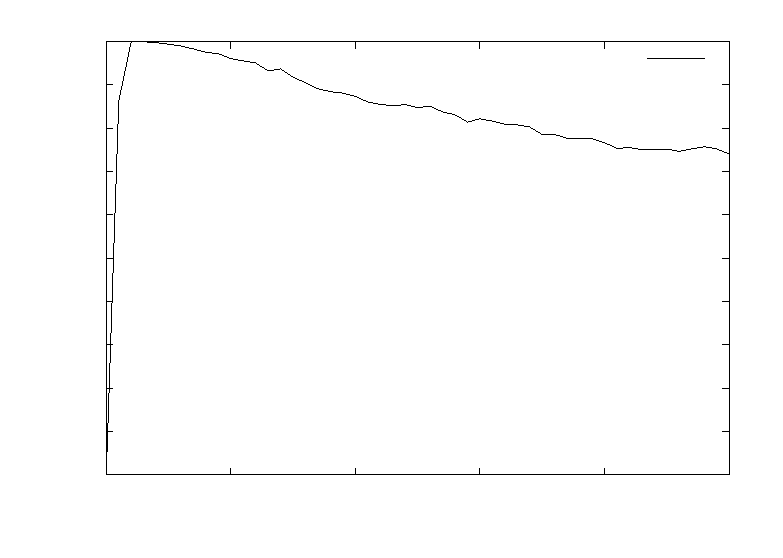
\includegraphics{chapters/chapter6/graphs/robustness/specializationratioovertime}}%
    \gplfronttext
  \end{picture}%
\endgroup
}
\caption{Specialization ratio over time, $\tau(t)$, of the honey bee algorithm, on a uniform environment, with environment item type ratio, $r=0.75$, and initial swarm specialization ratio, $\tau(0)=0$}
\label{fig:specializationratioovertime}
\end{figure}

Figure~\ref{fig:specializationratioovertime} shows that $\tau$ increased from 0 to 1 in 200 iterations, which suggests that the honey bee scout robots switched their specializations to search for prioritized items when the honey bee scout robots could not find any non-prioritized items. After 200 iterations, the specialization ratio steadily declined from 1 to 0.73. The final swarm specialization ratio, $\tau(10000)=0.73$, is nearly the same as the environment ratio, $r=0.75$, suggesting that the honey bee algorithm eventually adapted the specialization ratio to effectively forage the environment item type ratio of the given environment.

The above analysis of the behaviour of the honey bee algorithm supports the hypothesis that the honey bee algorithm's superior flexibility can be attributed to the algorithm's ability to adapt the swarm's specialization ratio (via the division of labour mechanism described above) to more efficiently forage an environment of a given environment item ratio.

Both the na\"ive algorithm and desert ant algorithm do not have the ability to adapt the initial swarm specialization to forage any environment ratio, which means that both algorithms are  less flexible than the honey bee algorithm. 

The desert ant algorithm is the least flexible, which indicates that the algorithm is sensitive to the choice in $\tau(0)$ for each environment type ratio $r$. Unlike the na\"ive algorithm, which has the worst efficiency over all experiments, a good choice of $\tau$ will allow the algorithm to forage the environment significantly better for a specific environment item ratio. Despite the desert ant algorithm outperforming the na\"ive algorithm in efficiency (refer to Section~\ref{results:efficiency}), the na\"ive algorithm is substantially more flexible than the desert ant algorithm. $F_r$ reveals that the na\"ive algorithm's performance is invariant under the variation of $\tau(0)$ on different environment item type ratios, resulting in a high level of flexibility. However, the na\"ive algorithm's flexibility is practically irrelevant given how poorly the algorithm performs on all environments. 


\subsubsection{Flexibility in terms of environment distributions}
\label{setup:flexibility:environmentdistributions}

Similar to $F_r$, the performance measure, $F_\epsilon$ (defined in Section~\ref{flexibility:environmentdistributions}), measures how well the swarm parameters yielding the best efficiency for environments with a specific environment distribution generalize across environments with different environment distributions, for a specific algorithm. Similar to $F_r$, the smaller $F_\epsilon$ is, the more flexible an algorithm is considered to be, and $F_\epsilon$ is also calculated based on the results of all experiments. The results summarized in Table~\ref{table:flexibility} indicate that the honey bee algorithm was the most flexible in terms of environment distribution, followed by the desert ant algorithm. The na\"ive algorithm was the least flexible.

The honey bee algorithm's superior flexibility suggests the following hypothesis: The honey bee algorithm's ability to adapt $\tau$ (described in Section~\ref{honeybeeforaging}) enables the swarm to more efficiently forage the differing environment ratios of the accessible environment (refer to Section~\ref{accessibleenvironment}) at any point during the foraging process.

To provide evidence for this hypothesis, an in-depth examination of the honey bee algorithm is performed on a Gaussian environment with a high density of items. The environment has a low ratio of prioritized items and a swarm which has a high initial swarm specialization ratio (i.e. most robots are initially set to forage prioritized items). Since the non-prioritized items surround the prioritized items, the swarm should first forage the non-prioritized items in order to get access to the prioritized items. Once the swarm can reach the prioritized items, the swarm should switch to foraging the prioritized items. The example Gaussian environment is illustrated in Figure~\ref{fig:gaussianhighdensityenv}. The white cells represent an empty cell, the dark cells represent the cells containing a non-prioritized item and the shaded cells represent the cells containing a prioritized item. 

\begin{figure}[htbp!]
    \centering
    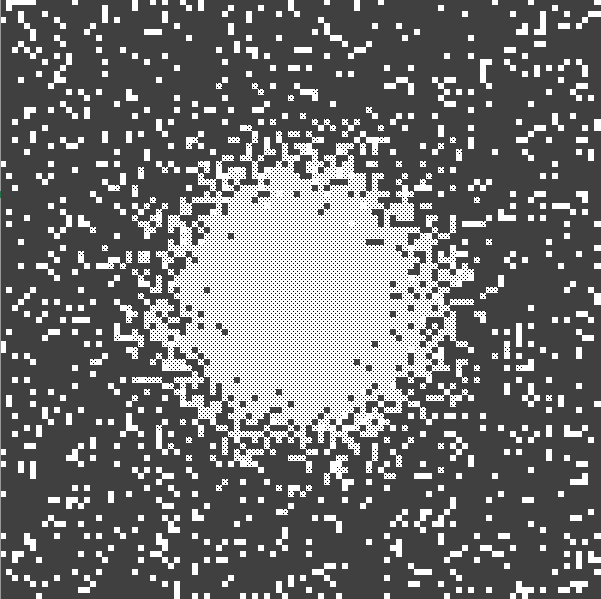
\includegraphics[width=0.75\textwidth]{figures/flexibility-gaussian-obj90-ratio.PNG}
    \caption{Gaussian environment with environment item type ratio, $r=0.2$, environment item density of $p=0.9$, and environment size $\Lambda=100$}
    \label{fig:gaussianhighdensityenv}
\end{figure}
    

The environment in Figure~\ref{fig:gaussianhighdensityenv} has the following properties:

\begin{itemize}
\item A Gaussian environment item distribution,
\item a low environmental item ratio of $r=0.2$,
\item a high density of items with $p=90$, and
\item an environment size, $\Lambda=100$.
\end{itemize}


Also, consider a swarm with the initial specialization ratio set to mostly forage prioritized items (i.e. $\tau(0)=0.8$) and with swarm density set to 0.5. The items nearest to the sink are all non-prioritized items. Robots will have to forage a large portion of the non-prioritized items between the sink and the centre of the environment in order to reach the high density of prioritized items at the centre of the environment. 


Figure~\ref{fig:gaussianhighdensityperformancehoneybee} shows the efficiency of foraging prioritized items, $E_P$, the efficiency of foraging non-prioritized items, $E_{NP}$, and specialization ratio over time, $\tau(t)$, for the honey bee algorithm on the environment described above. The performance measures were averaged over 30 independant runs.


\begin{figure}[!htbp]
\centering
\small
\resizebox{\textwidth}{!}{% GNUPLOT: LaTeX picture with Postscript
\begingroup
  \makeatletter
  \providecommand\color[2][]{%
    \GenericError{(gnuplot) \space\space\space\@spaces}{%
      Package color not loaded in conjunction with
      terminal option `colourtext'%
    }{See the gnuplot documentation for explanation.%
    }{Either use 'blacktext' in gnuplot or load the package
      color.sty in LaTeX.}%
    \renewcommand\color[2][]{}%
  }%
  \providecommand\includegraphics[2][]{%
    \GenericError{(gnuplot) \space\space\space\@spaces}{%
      Package graphicx or graphics not loaded%
    }{See the gnuplot documentation for explanation.%
    }{The gnuplot epslatex terminal needs graphicx.sty or graphics.sty.}%
    \renewcommand\includegraphics[2][]{}%
  }%
  \providecommand\rotatebox[2]{#2}%
  \@ifundefined{ifGPcolor}{%
    \newif\ifGPcolor
    \GPcolorfalse
  }{}%
  \@ifundefined{ifGPblacktext}{%
    \newif\ifGPblacktext
    \GPblacktexttrue
  }{}%
  % define a \g@addto@macro without @ in the name:
  \let\gplgaddtomacro\g@addto@macro
  % define empty templates for all commands taking text:
  \gdef\gplbacktext{}%
  \gdef\gplfronttext{}%
  \makeatother
  \ifGPblacktext
    % no textcolor at all
    \def\colorrgb#1{}%
    \def\colorgray#1{}%
  \else
    % gray or color?
    \ifGPcolor
      \def\colorrgb#1{\color[rgb]{#1}}%
      \def\colorgray#1{\color[gray]{#1}}%
      \expandafter\def\csname LTw\endcsname{\color{white}}%
      \expandafter\def\csname LTb\endcsname{\color{black}}%
      \expandafter\def\csname LTa\endcsname{\color{black}}%
      \expandafter\def\csname LT0\endcsname{\color[rgb]{1,0,0}}%
      \expandafter\def\csname LT1\endcsname{\color[rgb]{0,1,0}}%
      \expandafter\def\csname LT2\endcsname{\color[rgb]{0,0,1}}%
      \expandafter\def\csname LT3\endcsname{\color[rgb]{1,0,1}}%
      \expandafter\def\csname LT4\endcsname{\color[rgb]{0,1,1}}%
      \expandafter\def\csname LT5\endcsname{\color[rgb]{1,1,0}}%
      \expandafter\def\csname LT6\endcsname{\color[rgb]{0,0,0}}%
      \expandafter\def\csname LT7\endcsname{\color[rgb]{1,0.3,0}}%
      \expandafter\def\csname LT8\endcsname{\color[rgb]{0.5,0.5,0.5}}%
    \else
      % gray
      \def\colorrgb#1{\color{black}}%
      \def\colorgray#1{\color[gray]{#1}}%
      \expandafter\def\csname LTw\endcsname{\color{white}}%
      \expandafter\def\csname LTb\endcsname{\color{black}}%
      \expandafter\def\csname LTa\endcsname{\color{black}}%
      \expandafter\def\csname LT0\endcsname{\color{black}}%
      \expandafter\def\csname LT1\endcsname{\color{black}}%
      \expandafter\def\csname LT2\endcsname{\color{black}}%
      \expandafter\def\csname LT3\endcsname{\color{black}}%
      \expandafter\def\csname LT4\endcsname{\color{black}}%
      \expandafter\def\csname LT5\endcsname{\color{black}}%
      \expandafter\def\csname LT6\endcsname{\color{black}}%
      \expandafter\def\csname LT7\endcsname{\color{black}}%
      \expandafter\def\csname LT8\endcsname{\color{black}}%
    \fi
  \fi
    \setlength{\unitlength}{0.0500bp}%
    \ifx\gptboxheight\undefined%
      \newlength{\gptboxheight}%
      \newlength{\gptboxwidth}%
      \newsavebox{\gptboxtext}%
    \fi%
    \setlength{\fboxrule}{0.5pt}%
    \setlength{\fboxsep}{1pt}%
\begin{picture}(7200.00,5040.00)%
    \gplgaddtomacro\gplbacktext{%
      \csname LTb\endcsname%
      \put(740,640){\makebox(0,0)[r]{\strut{}$0$}}%
      \put(740,1020){\makebox(0,0)[r]{\strut{}$10$}}%
      \put(740,1400){\makebox(0,0)[r]{\strut{}$20$}}%
      \put(740,1780){\makebox(0,0)[r]{\strut{}$30$}}%
      \put(740,2160){\makebox(0,0)[r]{\strut{}$40$}}%
      \put(740,2540){\makebox(0,0)[r]{\strut{}$50$}}%
      \put(740,2919){\makebox(0,0)[r]{\strut{}$60$}}%
      \put(740,3299){\makebox(0,0)[r]{\strut{}$70$}}%
      \put(740,3679){\makebox(0,0)[r]{\strut{}$80$}}%
      \put(740,4059){\makebox(0,0)[r]{\strut{}$90$}}%
      \put(740,4439){\makebox(0,0)[r]{\strut{}$100$}}%
      \put(860,440){\makebox(0,0){\strut{}$0$}}%
      \put(1896,440){\makebox(0,0){\strut{}$2000$}}%
      \put(2932,440){\makebox(0,0){\strut{}$4000$}}%
      \put(3967,440){\makebox(0,0){\strut{}$6000$}}%
      \put(5003,440){\makebox(0,0){\strut{}$8000$}}%
      \put(6039,440){\makebox(0,0){\strut{}$10000$}}%
      \put(6159,640){\makebox(0,0)[l]{\strut{}$0$}}%
      \put(6159,1020){\makebox(0,0)[l]{\strut{}$0.1$}}%
      \put(6159,1400){\makebox(0,0)[l]{\strut{}$0.2$}}%
      \put(6159,1780){\makebox(0,0)[l]{\strut{}$0.3$}}%
      \put(6159,2160){\makebox(0,0)[l]{\strut{}$0.4$}}%
      \put(6159,2540){\makebox(0,0)[l]{\strut{}$0.5$}}%
      \put(6159,2919){\makebox(0,0)[l]{\strut{}$0.6$}}%
      \put(6159,3299){\makebox(0,0)[l]{\strut{}$0.7$}}%
      \put(6159,3679){\makebox(0,0)[l]{\strut{}$0.8$}}%
      \put(6159,4059){\makebox(0,0)[l]{\strut{}$0.9$}}%
      \put(6159,4439){\makebox(0,0)[l]{\strut{}$1$}}%
    }%
    \gplgaddtomacro\gplfronttext{%
      \csname LTb\endcsname%
      \put(160,2539){\rotatebox{-270}{\makebox(0,0){\strut{}Efficiency ($E_P$ and $E_{NP}$)}}}%
      \put(6738,2539){\rotatebox{-270}{\makebox(0,0){\strut{}Specialiation ratio, $\tau$}}}%
      \put(3449,140){\makebox(0,0){\strut{}time steps}}%
      \put(5136,4276){\makebox(0,0)[r]{\strut{}$E_P$}}%
      \put(5136,4076){\makebox(0,0)[r]{\strut{}$E_{NP}$}}%
      \put(5136,3876){\makebox(0,0)[r]{\strut{}$\tau$}}%
    }%
    \gplbacktext
    \put(0,0){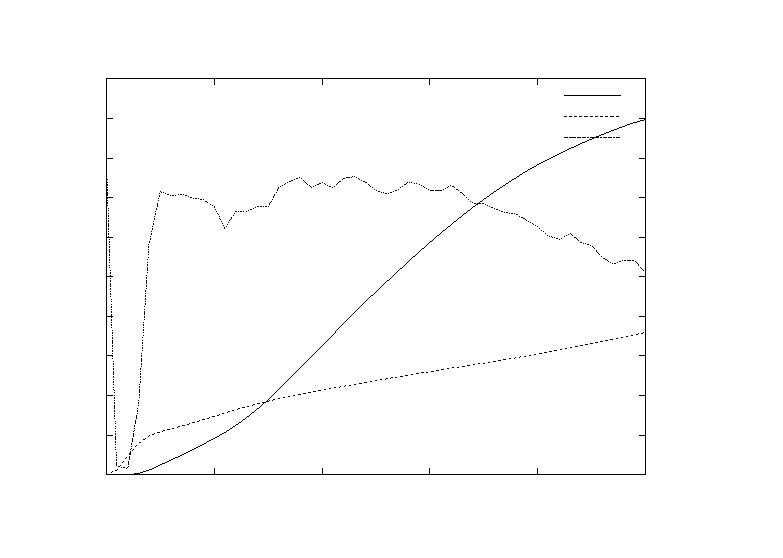
\includegraphics{chapters/chapter6/graphs/flexibility/flexibility-ED-gaussian-honeybee}}%
    \gplfronttext
  \end{picture}%
\endgroup
}
\caption{Efficiency of prioritized item foraging, $E_P$, efficiency of non-prioritized item foraging, $E_{NP}$, and specialization ratio over time, $\tau(t)$, for the honey bee algorithm on an example Gaussian environment, averaged over 30 independant runs}
\label{fig:gaussianhighdensityperformancehoneybee}
\end{figure}

In the first 200 time steps, the efficiency of foraging nonprioritized items, $E_{NP}$, increased very slowly. This was because there were very few robots that could forage non-prioritized items because most of the robots were initialized to forage prioritized items. The efficiency of foraging prioritized items, $E_{P}$, did not increase in the first 200 time steps, because the robots had no access to the prioritized items as they were blocked by the non-prioritized items. The initial specialization ratio, $\tau(0)$, that was initialized at 0.8, decreased very quickly to close to 0 in the first 200 time steps. The decrease in specialization ratio is good, because then most robots switched to forage non-prioritized items in the accessible environment which consisted entirely of non-prioritized items. Between 200 and 800 time steps, the $E_{NP}$ increased very quickly, due to the decrease in the swarm specialization ratio. The $E_{P}$ remained low between 200 and 800 time steps, because the prioritized items were not yet accessible to the swarm. After 800 time steps, $\tau$ increased from near 0 to just above 0.7, suggesting that the non-prioritized items have been cleared and the concentration of prioritized items in the centre have been reached. Thus, most of the robots in the swarm switched from foraging non-prioritized items to foraging prioritized items. The increase in swarm specialization ratio after 800 time steps was followed by a sharp increase in $E_P$. This demonstrated that the honey bee algorithm could adapt $\tau$ in order to initially forage the large number of non-prioritized items, and then switched to foraging mostly prioritized items when the prioritized items became accessible.

In constrast, the na\"ive algorithm's performance suffered because it lacks the ability to adapt swarm specialization. Figure~\ref{fig:gaussianhighdensityperformancenaive} illustrates the same performance measures, on the same Gaussian environment and swarm parameters for the na\"ive algorithm.  

Because the na\"ive algorithm does not enable robots to switch their item specialization, the swarm specialization ratio, $\tau$, remains constant. Because so few robots could clear non-prioritized items, due to the large initial swarm specialization ratio, $E_{NP}$ increased slowly throughout the experiment. Because the swarm was slow to clear the non-prioritized items, $E_P$ also remained small throughout the experiment, since the swarm struggled to make the prioritized items easily accessible. This suggests that prioritized foraging robots experienced environmental interference while attempting to navigate around the unforaged non-prioritized items. The rate of increase in $E_P$ increased over the duration of the experiment, as the swarm cleared more of the non-prioritized items. The behaviour for the desert ant algorithm was similar to that of the na\"ive algorithm, except that the final efficiency was greater for the desert ant algorithm.


\begin{figure}[!htbp]
\centering
\small
\resizebox{\textwidth}{!}{% GNUPLOT: LaTeX picture with Postscript
\begingroup
  \makeatletter
  \providecommand\color[2][]{%
    \GenericError{(gnuplot) \space\space\space\@spaces}{%
      Package color not loaded in conjunction with
      terminal option `colourtext'%
    }{See the gnuplot documentation for explanation.%
    }{Either use 'blacktext' in gnuplot or load the package
      color.sty in LaTeX.}%
    \renewcommand\color[2][]{}%
  }%
  \providecommand\includegraphics[2][]{%
    \GenericError{(gnuplot) \space\space\space\@spaces}{%
      Package graphicx or graphics not loaded%
    }{See the gnuplot documentation for explanation.%
    }{The gnuplot epslatex terminal needs graphicx.sty or graphics.sty.}%
    \renewcommand\includegraphics[2][]{}%
  }%
  \providecommand\rotatebox[2]{#2}%
  \@ifundefined{ifGPcolor}{%
    \newif\ifGPcolor
    \GPcolorfalse
  }{}%
  \@ifundefined{ifGPblacktext}{%
    \newif\ifGPblacktext
    \GPblacktexttrue
  }{}%
  % define a \g@addto@macro without @ in the name:
  \let\gplgaddtomacro\g@addto@macro
  % define empty templates for all commands taking text:
  \gdef\gplbacktext{}%
  \gdef\gplfronttext{}%
  \makeatother
  \ifGPblacktext
    % no textcolor at all
    \def\colorrgb#1{}%
    \def\colorgray#1{}%
  \else
    % gray or color?
    \ifGPcolor
      \def\colorrgb#1{\color[rgb]{#1}}%
      \def\colorgray#1{\color[gray]{#1}}%
      \expandafter\def\csname LTw\endcsname{\color{white}}%
      \expandafter\def\csname LTb\endcsname{\color{black}}%
      \expandafter\def\csname LTa\endcsname{\color{black}}%
      \expandafter\def\csname LT0\endcsname{\color[rgb]{1,0,0}}%
      \expandafter\def\csname LT1\endcsname{\color[rgb]{0,1,0}}%
      \expandafter\def\csname LT2\endcsname{\color[rgb]{0,0,1}}%
      \expandafter\def\csname LT3\endcsname{\color[rgb]{1,0,1}}%
      \expandafter\def\csname LT4\endcsname{\color[rgb]{0,1,1}}%
      \expandafter\def\csname LT5\endcsname{\color[rgb]{1,1,0}}%
      \expandafter\def\csname LT6\endcsname{\color[rgb]{0,0,0}}%
      \expandafter\def\csname LT7\endcsname{\color[rgb]{1,0.3,0}}%
      \expandafter\def\csname LT8\endcsname{\color[rgb]{0.5,0.5,0.5}}%
    \else
      % gray
      \def\colorrgb#1{\color{black}}%
      \def\colorgray#1{\color[gray]{#1}}%
      \expandafter\def\csname LTw\endcsname{\color{white}}%
      \expandafter\def\csname LTb\endcsname{\color{black}}%
      \expandafter\def\csname LTa\endcsname{\color{black}}%
      \expandafter\def\csname LT0\endcsname{\color{black}}%
      \expandafter\def\csname LT1\endcsname{\color{black}}%
      \expandafter\def\csname LT2\endcsname{\color{black}}%
      \expandafter\def\csname LT3\endcsname{\color{black}}%
      \expandafter\def\csname LT4\endcsname{\color{black}}%
      \expandafter\def\csname LT5\endcsname{\color{black}}%
      \expandafter\def\csname LT6\endcsname{\color{black}}%
      \expandafter\def\csname LT7\endcsname{\color{black}}%
      \expandafter\def\csname LT8\endcsname{\color{black}}%
    \fi
  \fi
    \setlength{\unitlength}{0.0500bp}%
    \ifx\gptboxheight\undefined%
      \newlength{\gptboxheight}%
      \newlength{\gptboxwidth}%
      \newsavebox{\gptboxtext}%
    \fi%
    \setlength{\fboxrule}{0.5pt}%
    \setlength{\fboxsep}{1pt}%
\begin{picture}(7200.00,5040.00)%
    \gplgaddtomacro\gplbacktext{%
      \csname LTb\endcsname%
      \put(740,640){\makebox(0,0)[r]{\strut{}$0$}}%
      \put(740,1056){\makebox(0,0)[r]{\strut{}$10$}}%
      \put(740,1472){\makebox(0,0)[r]{\strut{}$20$}}%
      \put(740,1888){\makebox(0,0)[r]{\strut{}$30$}}%
      \put(740,2304){\makebox(0,0)[r]{\strut{}$40$}}%
      \put(740,2720){\makebox(0,0)[r]{\strut{}$50$}}%
      \put(740,3135){\makebox(0,0)[r]{\strut{}$60$}}%
      \put(740,3551){\makebox(0,0)[r]{\strut{}$70$}}%
      \put(740,3967){\makebox(0,0)[r]{\strut{}$80$}}%
      \put(740,4383){\makebox(0,0)[r]{\strut{}$90$}}%
      \put(740,4799){\makebox(0,0)[r]{\strut{}$100$}}%
      \put(860,440){\makebox(0,0){\strut{}$0$}}%
      \put(1896,440){\makebox(0,0){\strut{}$2000$}}%
      \put(2932,440){\makebox(0,0){\strut{}$4000$}}%
      \put(3967,440){\makebox(0,0){\strut{}$6000$}}%
      \put(5003,440){\makebox(0,0){\strut{}$8000$}}%
      \put(6039,440){\makebox(0,0){\strut{}$10000$}}%
      \put(6159,640){\makebox(0,0)[l]{\strut{}$0$}}%
      \put(6159,1056){\makebox(0,0)[l]{\strut{}$0.1$}}%
      \put(6159,1472){\makebox(0,0)[l]{\strut{}$0.2$}}%
      \put(6159,1888){\makebox(0,0)[l]{\strut{}$0.3$}}%
      \put(6159,2304){\makebox(0,0)[l]{\strut{}$0.4$}}%
      \put(6159,2720){\makebox(0,0)[l]{\strut{}$0.5$}}%
      \put(6159,3135){\makebox(0,0)[l]{\strut{}$0.6$}}%
      \put(6159,3551){\makebox(0,0)[l]{\strut{}$0.7$}}%
      \put(6159,3967){\makebox(0,0)[l]{\strut{}$0.8$}}%
      \put(6159,4383){\makebox(0,0)[l]{\strut{}$0.9$}}%
      \put(6159,4799){\makebox(0,0)[l]{\strut{}$1$}}%
    }%
    \gplgaddtomacro\gplfronttext{%
      \csname LTb\endcsname%
      \put(160,2719){\rotatebox{-270}{\makebox(0,0){\strut{}Efficiency}}}%
      \put(6738,2719){\rotatebox{-270}{\makebox(0,0){\strut{}Specialiation ratio, $\tau$}}}%
      \put(3449,140){\makebox(0,0){\strut{}time steps ($t$)}}%
      \put(5136,4636){\makebox(0,0)[r]{\strut{}$E_P$}}%
      \put(5136,4436){\makebox(0,0)[r]{\strut{}$E_{NP}$}}%
      \put(5136,4236){\makebox(0,0)[r]{\strut{}$\tau$}}%
    }%
    \gplbacktext
    \put(0,0){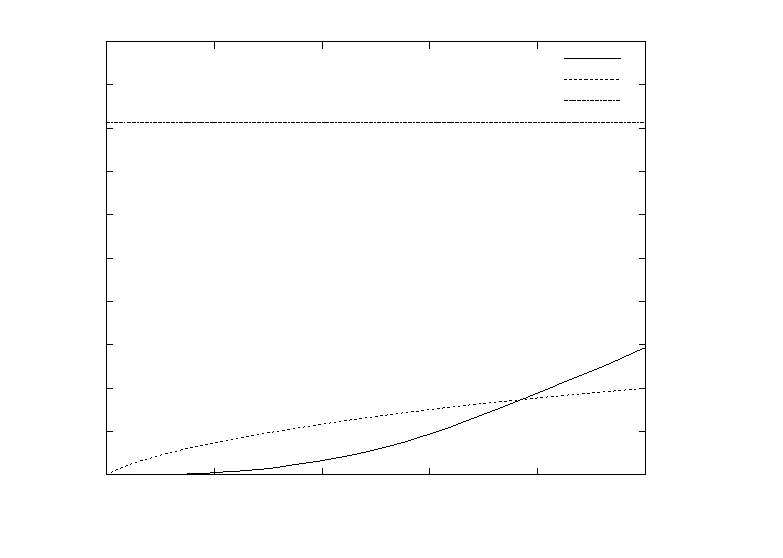
\includegraphics{graphs/flexibility/flexibility-ED-gaussian-naive}}%
    \gplfronttext
  \end{picture}%
\endgroup
}
\caption{Efficiency of prioritized item foraging, $E_P$, efficiency of non-prioritized item foraging, $E_{NP}$, and the specialization ratio over time, $\tau(t)$, for the na\"ive algorithm on a Gaussian evironment, averaged over 30 independant runs}
\label{fig:gaussianhighdensityperformancenaive}
\end{figure}

\begin{figure}[!htb]
\centering
\small
\resizebox{\textwidth}{!}{% GNUPLOT: LaTeX picture with Postscript
\begingroup
  \makeatletter
  \providecommand\color[2][]{%
    \GenericError{(gnuplot) \space\space\space\@spaces}{%
      Package color not loaded in conjunction with
      terminal option `colourtext'%
    }{See the gnuplot documentation for explanation.%
    }{Either use 'blacktext' in gnuplot or load the package
      color.sty in LaTeX.}%
    \renewcommand\color[2][]{}%
  }%
  \providecommand\includegraphics[2][]{%
    \GenericError{(gnuplot) \space\space\space\@spaces}{%
      Package graphicx or graphics not loaded%
    }{See the gnuplot documentation for explanation.%
    }{The gnuplot epslatex terminal needs graphicx.sty or graphics.sty.}%
    \renewcommand\includegraphics[2][]{}%
  }%
  \providecommand\rotatebox[2]{#2}%
  \@ifundefined{ifGPcolor}{%
    \newif\ifGPcolor
    \GPcolorfalse
  }{}%
  \@ifundefined{ifGPblacktext}{%
    \newif\ifGPblacktext
    \GPblacktexttrue
  }{}%
  % define a \g@addto@macro without @ in the name:
  \let\gplgaddtomacro\g@addto@macro
  % define empty templates for all commands taking text:
  \gdef\gplbacktext{}%
  \gdef\gplfronttext{}%
  \makeatother
  \ifGPblacktext
    % no textcolor at all
    \def\colorrgb#1{}%
    \def\colorgray#1{}%
  \else
    % gray or color?
    \ifGPcolor
      \def\colorrgb#1{\color[rgb]{#1}}%
      \def\colorgray#1{\color[gray]{#1}}%
      \expandafter\def\csname LTw\endcsname{\color{white}}%
      \expandafter\def\csname LTb\endcsname{\color{black}}%
      \expandafter\def\csname LTa\endcsname{\color{black}}%
      \expandafter\def\csname LT0\endcsname{\color[rgb]{1,0,0}}%
      \expandafter\def\csname LT1\endcsname{\color[rgb]{0,1,0}}%
      \expandafter\def\csname LT2\endcsname{\color[rgb]{0,0,1}}%
      \expandafter\def\csname LT3\endcsname{\color[rgb]{1,0,1}}%
      \expandafter\def\csname LT4\endcsname{\color[rgb]{0,1,1}}%
      \expandafter\def\csname LT5\endcsname{\color[rgb]{1,1,0}}%
      \expandafter\def\csname LT6\endcsname{\color[rgb]{0,0,0}}%
      \expandafter\def\csname LT7\endcsname{\color[rgb]{1,0.3,0}}%
      \expandafter\def\csname LT8\endcsname{\color[rgb]{0.5,0.5,0.5}}%
    \else
      % gray
      \def\colorrgb#1{\color{black}}%
      \def\colorgray#1{\color[gray]{#1}}%
      \expandafter\def\csname LTw\endcsname{\color{white}}%
      \expandafter\def\csname LTb\endcsname{\color{black}}%
      \expandafter\def\csname LTa\endcsname{\color{black}}%
      \expandafter\def\csname LT0\endcsname{\color{black}}%
      \expandafter\def\csname LT1\endcsname{\color{black}}%
      \expandafter\def\csname LT2\endcsname{\color{black}}%
      \expandafter\def\csname LT3\endcsname{\color{black}}%
      \expandafter\def\csname LT4\endcsname{\color{black}}%
      \expandafter\def\csname LT5\endcsname{\color{black}}%
      \expandafter\def\csname LT6\endcsname{\color{black}}%
      \expandafter\def\csname LT7\endcsname{\color{black}}%
      \expandafter\def\csname LT8\endcsname{\color{black}}%
    \fi
  \fi
    \setlength{\unitlength}{0.0500bp}%
    \ifx\gptboxheight\undefined%
      \newlength{\gptboxheight}%
      \newlength{\gptboxwidth}%
      \newsavebox{\gptboxtext}%
    \fi%
    \setlength{\fboxrule}{0.5pt}%
    \setlength{\fboxsep}{1pt}%
\begin{picture}(7200.00,5040.00)%
    \gplgaddtomacro\gplbacktext{%
      \csname LTb\endcsname%
      \put(740,640){\makebox(0,0)[r]{\strut{}$0$}}%
      \put(740,1020){\makebox(0,0)[r]{\strut{}$10$}}%
      \put(740,1400){\makebox(0,0)[r]{\strut{}$20$}}%
      \put(740,1780){\makebox(0,0)[r]{\strut{}$30$}}%
      \put(740,2160){\makebox(0,0)[r]{\strut{}$40$}}%
      \put(740,2540){\makebox(0,0)[r]{\strut{}$50$}}%
      \put(740,2919){\makebox(0,0)[r]{\strut{}$60$}}%
      \put(740,3299){\makebox(0,0)[r]{\strut{}$70$}}%
      \put(740,3679){\makebox(0,0)[r]{\strut{}$80$}}%
      \put(740,4059){\makebox(0,0)[r]{\strut{}$90$}}%
      \put(740,4439){\makebox(0,0)[r]{\strut{}$100$}}%
      \put(860,440){\makebox(0,0){\strut{}$0$}}%
      \put(1896,440){\makebox(0,0){\strut{}$2000$}}%
      \put(2932,440){\makebox(0,0){\strut{}$4000$}}%
      \put(3967,440){\makebox(0,0){\strut{}$6000$}}%
      \put(5003,440){\makebox(0,0){\strut{}$8000$}}%
      \put(6039,440){\makebox(0,0){\strut{}$10000$}}%
      \put(6159,640){\makebox(0,0)[l]{\strut{}$0$}}%
      \put(6159,1020){\makebox(0,0)[l]{\strut{}$0.1$}}%
      \put(6159,1400){\makebox(0,0)[l]{\strut{}$0.2$}}%
      \put(6159,1780){\makebox(0,0)[l]{\strut{}$0.3$}}%
      \put(6159,2160){\makebox(0,0)[l]{\strut{}$0.4$}}%
      \put(6159,2540){\makebox(0,0)[l]{\strut{}$0.5$}}%
      \put(6159,2919){\makebox(0,0)[l]{\strut{}$0.6$}}%
      \put(6159,3299){\makebox(0,0)[l]{\strut{}$0.7$}}%
      \put(6159,3679){\makebox(0,0)[l]{\strut{}$0.8$}}%
      \put(6159,4059){\makebox(0,0)[l]{\strut{}$0.9$}}%
      \put(6159,4439){\makebox(0,0)[l]{\strut{}$1$}}%
    }%
    \gplgaddtomacro\gplfronttext{%
      \csname LTb\endcsname%
      \put(160,2539){\rotatebox{-270}{\makebox(0,0){\strut{}Efficiency}}}%
      \put(6738,2539){\rotatebox{-270}{\makebox(0,0){\strut{}Specialiation ratio, $\tau$}}}%
      \put(3449,140){\makebox(0,0){\strut{}iteration}}%
      \put(3449,4739){\makebox(0,0){\strut{}Efficiency of prioritized item foraging $E_P$, Efficiency of non-prioritized item foraging $E_{NP}$, Specialization ratio $\tau$ over time, for Honey Bee in Uniform Environment}}%
      \put(5136,4276){\makebox(0,0)[r]{\strut{}$E_P$}}%
      \put(5136,4076){\makebox(0,0)[r]{\strut{}$E_{NP}$}}%
      \put(5136,3876){\makebox(0,0)[r]{\strut{}$\tau$}}%
    }%
    \gplbacktext
    \put(0,0){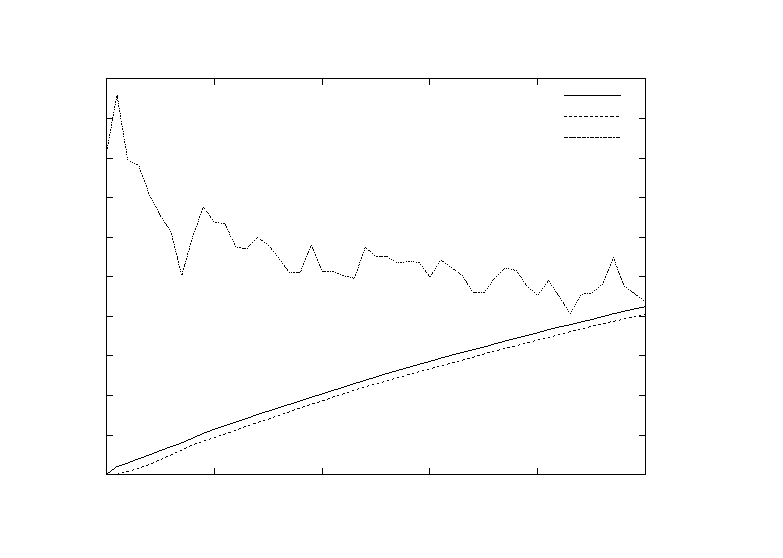
\includegraphics{chapters/chapter6/graphs/flexibility/flexibility-ED-uniform-honeybee}}%
    \gplfronttext
  \end{picture}%
\endgroup
}
\caption{Efficiency of prioritized item foraging, $E_P$, over time $t$, efficiency of non-prioritized item foraging, $E_{NP}$, over time $t$, and specialization ratio, $\tau(t)$, for the honey bee algorithm on a uniform environment, averaged over 30 independant runs}
\label{fig:uniformhighdensityperformancehoneybee}
\end{figure}


Figure~\ref{fig:gaussianhighdensityperformancehoneybee} shows that the final $E_P$ for the honey bee algorithm, averaged over 30 independant runs, was 0.9, while Figure~\ref{fig:gaussianhighdensityperformancenaive} shows that the final $E_P$ for the na\"ive algorithm was only 0.3. Since the honey bee algorithm adapts $\tau$, the honey bee algorithm shows an increased ability to forage obstacles (the non-prioritized items) in order to more easily access hard to reach prioritized items. As a result, the honey bee algorithm is more flexible to different environment distributions than the na\"ive or desert ant algorithms.


To provide further evidence for the above hypothesis, consider other environment distributions to show that the honey bee algorithm can adapt the swarm's swarm specialization ratio appropriately for different distributions. Thus, consider a uniform environment with the same environment parameters as above. Because the environment distribution is uniform, the environment ratio of the accessible environment will fluctuate erratically as the swarm forages the environment.  

Figure~\ref{fig:uniformhighdensityperformancehoneybee} shows the same performance measures for an experiment with the same swarm parameters as above on the uniform environment for the honey bee algorithm. The specialization ratio has a downward erratic trend, from over 0.9 to approximately 0.4. The erratic fluctuation of $\tau$ is due to minor and short-lived erratic differences in the environment ratio of the accessible environment which would feature in uniform environments. The rates of foraging efficiency, $E_P$ and $E_{NP}$, increase constantly throughout the experiment. 

The above analysis provides evidence for the hypothesis that suggests that the honey bee algorithm is capable of adapting the swarm to forage the accessible environment. Thus the honey bee algorithm has higher flexibility on different environment distributions compared to the desert ant and na\"ive algorithms. The desert ant and na\"ive algorithms have more difficulty foraging certain distributions as they cannot adapt $\tau$ to more effectively forage the accessible environment.

Table~\ref{table:flexibility} indicates that the desert ant algorithm is more flexible over environment distributions than the the na\"ive algorithm. Considering the fact that the only difference between the na\"ive algorithm and the desert ant algorithm is the fact that the desert ant algorithm uses site fidelity while the na\"ive algorithm does not, the difference in performance must be attributed to the desert ant's use of site fidelity. %TODO: How about we examine the vein environment? Dessert ant could use site fidelity. 

\subsection{Scalability}
\label{results:scalability}

This section discusses the scalability of each algorithm in terms of the macro performance measures: swarm density and problem complexity. Section~\ref{results:swarmscalability} discusses the scalability of each algorithm in terms of swarm density, while Section~\ref{results:problemscalability} evaluates the scalability of each algorithm in terms of the complexity of the problem.

\subsubsection{Swarm scalability}
\label{results:swarmscalability}

Table~\ref{table:swarmscalability} presents the swarm density scalability results, $S_c$. Figure~\ref{fig:swarmscalability} shows the swarm density scalability for each density, $S_{c_i}$, for each algorithm (as defined Section~\ref{swarmsizescalability}). The na\"ive algorithm was the most scalable while the desert ant and the honey bee algorithms show similar scalability. The honey bee algorithm is more scalable than the desert ant algorithm for $c < 0.9$, but at $c \geq 0.9$, the swarm scalability, $S_{c_i}$, of the desert ant algorithm was greater than the honey bee algorithm.

\begin{table}[!htbp]
\centering
\caption{Swarm scalability, $S_{c_i}$, for each swarm density in $\overline{c}$, for each algorithm.}
\label{table:swarmscalability}
\begin{tabular}{@{}lllllll@{}}
\toprule
\textbf{$c$}            & \textbf{0.1} & \textbf{0.3}         & \textbf{0.5}         & \textbf{0.7}         & \textbf{1}           \\ \midrule
\textbf{na\"ive}    & 1   & 2.148 & 2.951  & 3.568 & 4.255  \\
\textbf{desert ant} & 1   & 1.973 & 2.605 & 3.058  & 3.556 \\
\textbf{honey bee}  & 1   & 2.067 & 2.706 & 3.119 & 3.532 \\ \bottomrule
\end{tabular}
\end{table}

\begin{figure}[!htbp]
\centering
\small
\resizebox{\textwidth}{!}{% GNUPLOT: LaTeX picture with Postscript
\begingroup
  \makeatletter
  \providecommand\color[2][]{%
    \GenericError{(gnuplot) \space\space\space\@spaces}{%
      Package color not loaded in conjunction with
      terminal option `colourtext'%
    }{See the gnuplot documentation for explanation.%
    }{Either use 'blacktext' in gnuplot or load the package
      color.sty in LaTeX.}%
    \renewcommand\color[2][]{}%
  }%
  \providecommand\includegraphics[2][]{%
    \GenericError{(gnuplot) \space\space\space\@spaces}{%
      Package graphicx or graphics not loaded%
    }{See the gnuplot documentation for explanation.%
    }{The gnuplot epslatex terminal needs graphicx.sty or graphics.sty.}%
    \renewcommand\includegraphics[2][]{}%
  }%
  \providecommand\rotatebox[2]{#2}%
  \@ifundefined{ifGPcolor}{%
    \newif\ifGPcolor
    \GPcolorfalse
  }{}%
  \@ifundefined{ifGPblacktext}{%
    \newif\ifGPblacktext
    \GPblacktexttrue
  }{}%
  % define a \g@addto@macro without @ in the name:
  \let\gplgaddtomacro\g@addto@macro
  % define empty templates for all commands taking text:
  \gdef\gplbacktext{}%
  \gdef\gplfronttext{}%
  \makeatother
  \ifGPblacktext
    % no textcolor at all
    \def\colorrgb#1{}%
    \def\colorgray#1{}%
  \else
    % gray or color?
    \ifGPcolor
      \def\colorrgb#1{\color[rgb]{#1}}%
      \def\colorgray#1{\color[gray]{#1}}%
      \expandafter\def\csname LTw\endcsname{\color{white}}%
      \expandafter\def\csname LTb\endcsname{\color{black}}%
      \expandafter\def\csname LTa\endcsname{\color{black}}%
      \expandafter\def\csname LT0\endcsname{\color[rgb]{1,0,0}}%
      \expandafter\def\csname LT1\endcsname{\color[rgb]{0,1,0}}%
      \expandafter\def\csname LT2\endcsname{\color[rgb]{0,0,1}}%
      \expandafter\def\csname LT3\endcsname{\color[rgb]{1,0,1}}%
      \expandafter\def\csname LT4\endcsname{\color[rgb]{0,1,1}}%
      \expandafter\def\csname LT5\endcsname{\color[rgb]{1,1,0}}%
      \expandafter\def\csname LT6\endcsname{\color[rgb]{0,0,0}}%
      \expandafter\def\csname LT7\endcsname{\color[rgb]{1,0.3,0}}%
      \expandafter\def\csname LT8\endcsname{\color[rgb]{0.5,0.5,0.5}}%
    \else
      % gray
      \def\colorrgb#1{\color{black}}%
      \def\colorgray#1{\color[gray]{#1}}%
      \expandafter\def\csname LTw\endcsname{\color{white}}%
      \expandafter\def\csname LTb\endcsname{\color{black}}%
      \expandafter\def\csname LTa\endcsname{\color{black}}%
      \expandafter\def\csname LT0\endcsname{\color{black}}%
      \expandafter\def\csname LT1\endcsname{\color{black}}%
      \expandafter\def\csname LT2\endcsname{\color{black}}%
      \expandafter\def\csname LT3\endcsname{\color{black}}%
      \expandafter\def\csname LT4\endcsname{\color{black}}%
      \expandafter\def\csname LT5\endcsname{\color{black}}%
      \expandafter\def\csname LT6\endcsname{\color{black}}%
      \expandafter\def\csname LT7\endcsname{\color{black}}%
      \expandafter\def\csname LT8\endcsname{\color{black}}%
    \fi
  \fi
    \setlength{\unitlength}{0.0500bp}%
    \ifx\gptboxheight\undefined%
      \newlength{\gptboxheight}%
      \newlength{\gptboxwidth}%
      \newsavebox{\gptboxtext}%
    \fi%
    \setlength{\fboxrule}{0.5pt}%
    \setlength{\fboxsep}{1pt}%
\begin{picture}(7200.00,5040.00)%
    \gplgaddtomacro\gplbacktext{%
      \csname LTb\endcsname%
      \put(620,640){\makebox(0,0)[r]{\strut{}$1$}}%
      \put(620,1062){\makebox(0,0)[r]{\strut{}$2$}}%
      \put(620,1484){\makebox(0,0)[r]{\strut{}$3$}}%
      \put(620,1906){\makebox(0,0)[r]{\strut{}$4$}}%
      \put(620,2328){\makebox(0,0)[r]{\strut{}$5$}}%
      \put(620,2751){\makebox(0,0)[r]{\strut{}$6$}}%
      \put(620,3173){\makebox(0,0)[r]{\strut{}$7$}}%
      \put(620,3595){\makebox(0,0)[r]{\strut{}$8$}}%
      \put(620,4017){\makebox(0,0)[r]{\strut{}$9$}}%
      \put(620,4439){\makebox(0,0)[r]{\strut{}$10$}}%
      \put(740,440){\makebox(0,0){\strut{}$0.1$}}%
      \put(1418,440){\makebox(0,0){\strut{}$0.2$}}%
      \put(2095,440){\makebox(0,0){\strut{}$0.3$}}%
      \put(2773,440){\makebox(0,0){\strut{}$0.4$}}%
      \put(3451,440){\makebox(0,0){\strut{}$0.5$}}%
      \put(4128,440){\makebox(0,0){\strut{}$0.6$}}%
      \put(4806,440){\makebox(0,0){\strut{}$0.7$}}%
      \put(5484,440){\makebox(0,0){\strut{}$0.8$}}%
      \put(6161,440){\makebox(0,0){\strut{}$0.9$}}%
      \put(6839,440){\makebox(0,0){\strut{}$1$}}%
    }%
    \gplgaddtomacro\gplfronttext{%
      \csname LTb\endcsname%
      \put(160,2539){\rotatebox{-270}{\makebox(0,0){\strut{}Swarm Scalability ($SS$)}}}%
      \put(3789,140){\makebox(0,0){\strut{}swarm density ($c$)}}%
      \put(3789,4739){\makebox(0,0){\strut{}Swarm Scalability, $SS$, for each swarm density $c$, for each algorithm}}%
      \put(5936,4276){\makebox(0,0)[r]{\strut{}Na\"ive}}%
      \put(5936,4076){\makebox(0,0)[r]{\strut{}Desert Ant}}%
      \put(5936,3876){\makebox(0,0)[r]{\strut{}Honey Bee}}%
      \put(5936,3676){\makebox(0,0)[r]{\strut{}Linear Scalability}}%
    }%
    \gplbacktext
    \put(0,0){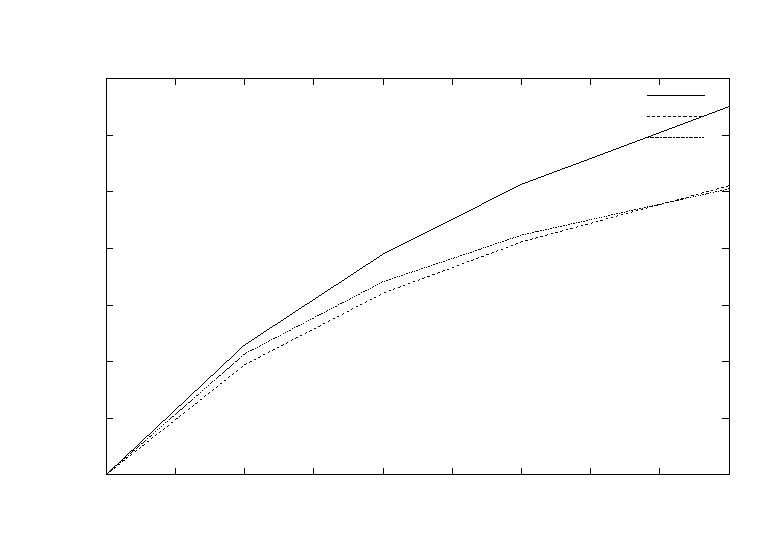
\includegraphics{chapters/chapter6/graphs/scalability/swarmscalability}}%
    \gplfronttext
  \end{picture}%
\endgroup
}
\caption{Swarm scalability, $S_c$, for each swarm density $c_i$ in $\overline{c}$ for each algorithm.}
\label{fig:swarmscalability}
\end{figure}

Figure~\ref{fig:swarmscalability} also plots the ideal scalability. Ideal scalability is when the increase in swarm density is directly proportional to the increase in efficiency. The ideal values for $S_{c_i}$ were calculated and plotted. All algorithms fall below the ideal scalability line and thus have sublinear (logarithmic) scalability. Section~\ref{swarmsizescalability} highlighted that increased inter-robot interference is a major factor that impacts on swarm scalability. It can be concluded that the reason for sub-linear performance in all algorithms was because all algorithms suffer from increased inter-robot interference as swarm size increases.

To understand why the desert ant and the honey bee algorithms were less scalable than the na\"ive algorithm, consider the following: The na\"ive algorithm, being the most simple foraging algorithm, has no mechanism to enable the swarm to exploit high quality sites of prioritized items and can only locate items by randomly exploring the environment. Both the desert ant algorithm and the honey bee algorithm have mechanisms to exploit high quality areas: The desert ant algorithm uses site fidelity and the honey bee algorithm uses recruitment to exploit high quality sites. 

Suppose that there exists a single high quality site in an environment. Using site-fidelity and recruitment, the desert ant and the honey bee algorithms can exploit that high quality area. In exploiting that high quality site, the path between the sink and the high-quality site becomes more congested as more robots share the path between the sink and the high quality area. The increased congestion on that path will cause more inter-robot interference. However, due to the focused efforts of the swarm on a high quality area of the environment, the exploitation will still improve foraging efficiency overall, compared to the na\"ive algorithm at low swarm densities. However, as swarm density increases, the congestion on the route between the high quality site and the sink will increase, hindering foraging efficiency due to increased inter-robot interference. It follows that the desert ant algorithm and the honey bee algorithm are less scalable in terms of swarm density than the na\"ive algorithm, due to the increased inter-robot interference as a result of exploitation of high quality sites.

The recruitment mechanism used by the honey bee algorithm is a more extreme form of exploitation than site fidelity used by the desert ant algorithm, because scouts recruit groups of robots to forage single areas. On the other hand, when using site fidelity, the high quality site is only foraged by the robot that found it. Considering that the recruitment mechanism is more exploitative than the site fidelity mechanism, one would expect the honey bee algorithm to be much less scalable than the desert ant algorithm, but that is not demonstrated in Table~\ref{table:swarmscalability}. Instead, the honey bee algorithm performed slightly better than the desert ant algorithm for all $c < 0.8$.

To explain the honey bee algorithm's ability to outperform the desert ant algorithm at most swarm densities, consider the honey bee algorithm's division of labour mechanism as described in Section~\ref{honeybeeforaging}. The division of labour mechanism will cause an active forager robot to return to the sink if that robot can not find an item for a maximum amount of time. The inactive forager robot waits at the sink, until the inactive forager robot is recruited by a scout robot. Section~\ref{background:divisionoflabour:robotswarm} discussed that a mechanism of division of labour which could adjust the number of robots actively foraging to an appropriate number, would result in decreased levels of inter-robot interference and increased swarm scalability.

In order to determine whether the slight improvement in scalability of the honey bee algorithm over the desert ant algorithm can be attributed to the discussed division of labour mechanism, the average time spent by robots in the waiting state is plotted for different values of $c$ in Figure~\ref{fig:swarmscalabilitywaitingtime}. Figure~\ref{fig:swarmscalabilitywaitingtime} illustrates that the robots spend a significant portion of time in the waiting state for $c < 0.5$, which provides evidence that the honey bee algorithm's swarm scalability is greater than the desert ant algorithm's swarm scalability for low values of $c$.

\begin{figure}[!htbp]
\centering
\small
\resizebox{\textwidth}{!}{% GNUPLOT: LaTeX picture with Postscript
\begingroup
  \makeatletter
  \providecommand\color[2][]{%
    \GenericError{(gnuplot) \space\space\space\@spaces}{%
      Package color not loaded in conjunction with
      terminal option `colourtext'%
    }{See the gnuplot documentation for explanation.%
    }{Either use 'blacktext' in gnuplot or load the package
      color.sty in LaTeX.}%
    \renewcommand\color[2][]{}%
  }%
  \providecommand\includegraphics[2][]{%
    \GenericError{(gnuplot) \space\space\space\@spaces}{%
      Package graphicx or graphics not loaded%
    }{See the gnuplot documentation for explanation.%
    }{The gnuplot epslatex terminal needs graphicx.sty or graphics.sty.}%
    \renewcommand\includegraphics[2][]{}%
  }%
  \providecommand\rotatebox[2]{#2}%
  \@ifundefined{ifGPcolor}{%
    \newif\ifGPcolor
    \GPcolorfalse
  }{}%
  \@ifundefined{ifGPblacktext}{%
    \newif\ifGPblacktext
    \GPblacktexttrue
  }{}%
  % define a \g@addto@macro without @ in the name:
  \let\gplgaddtomacro\g@addto@macro
  % define empty templates for all commands taking text:
  \gdef\gplbacktext{}%
  \gdef\gplfronttext{}%
  \makeatother
  \ifGPblacktext
    % no textcolor at all
    \def\colorrgb#1{}%
    \def\colorgray#1{}%
  \else
    % gray or color?
    \ifGPcolor
      \def\colorrgb#1{\color[rgb]{#1}}%
      \def\colorgray#1{\color[gray]{#1}}%
      \expandafter\def\csname LTw\endcsname{\color{white}}%
      \expandafter\def\csname LTb\endcsname{\color{black}}%
      \expandafter\def\csname LTa\endcsname{\color{black}}%
      \expandafter\def\csname LT0\endcsname{\color[rgb]{1,0,0}}%
      \expandafter\def\csname LT1\endcsname{\color[rgb]{0,1,0}}%
      \expandafter\def\csname LT2\endcsname{\color[rgb]{0,0,1}}%
      \expandafter\def\csname LT3\endcsname{\color[rgb]{1,0,1}}%
      \expandafter\def\csname LT4\endcsname{\color[rgb]{0,1,1}}%
      \expandafter\def\csname LT5\endcsname{\color[rgb]{1,1,0}}%
      \expandafter\def\csname LT6\endcsname{\color[rgb]{0,0,0}}%
      \expandafter\def\csname LT7\endcsname{\color[rgb]{1,0.3,0}}%
      \expandafter\def\csname LT8\endcsname{\color[rgb]{0.5,0.5,0.5}}%
    \else
      % gray
      \def\colorrgb#1{\color{black}}%
      \def\colorgray#1{\color[gray]{#1}}%
      \expandafter\def\csname LTw\endcsname{\color{white}}%
      \expandafter\def\csname LTb\endcsname{\color{black}}%
      \expandafter\def\csname LTa\endcsname{\color{black}}%
      \expandafter\def\csname LT0\endcsname{\color{black}}%
      \expandafter\def\csname LT1\endcsname{\color{black}}%
      \expandafter\def\csname LT2\endcsname{\color{black}}%
      \expandafter\def\csname LT3\endcsname{\color{black}}%
      \expandafter\def\csname LT4\endcsname{\color{black}}%
      \expandafter\def\csname LT5\endcsname{\color{black}}%
      \expandafter\def\csname LT6\endcsname{\color{black}}%
      \expandafter\def\csname LT7\endcsname{\color{black}}%
      \expandafter\def\csname LT8\endcsname{\color{black}}%
    \fi
  \fi
    \setlength{\unitlength}{0.0500bp}%
    \ifx\gptboxheight\undefined%
      \newlength{\gptboxheight}%
      \newlength{\gptboxwidth}%
      \newsavebox{\gptboxtext}%
    \fi%
    \setlength{\fboxrule}{0.5pt}%
    \setlength{\fboxsep}{1pt}%
\begin{picture}(7200.00,5040.00)%
    \gplgaddtomacro\gplbacktext{%
      \csname LTb\endcsname%
      \put(860,640){\makebox(0,0)[r]{\strut{}$0.05$}}%
      \put(860,1400){\makebox(0,0)[r]{\strut{}$0.1$}}%
      \put(860,2160){\makebox(0,0)[r]{\strut{}$0.15$}}%
      \put(860,2919){\makebox(0,0)[r]{\strut{}$0.2$}}%
      \put(860,3679){\makebox(0,0)[r]{\strut{}$0.25$}}%
      \put(860,4439){\makebox(0,0)[r]{\strut{}$0.3$}}%
      \put(980,440){\makebox(0,0){\strut{}$0.1$}}%
      \put(1631,440){\makebox(0,0){\strut{}$0.2$}}%
      \put(2282,440){\makebox(0,0){\strut{}$0.3$}}%
      \put(2933,440){\makebox(0,0){\strut{}$0.4$}}%
      \put(3584,440){\makebox(0,0){\strut{}$0.5$}}%
      \put(4235,440){\makebox(0,0){\strut{}$0.6$}}%
      \put(4886,440){\makebox(0,0){\strut{}$0.7$}}%
      \put(5537,440){\makebox(0,0){\strut{}$0.8$}}%
      \put(6188,440){\makebox(0,0){\strut{}$0.9$}}%
      \put(6839,440){\makebox(0,0){\strut{}$1$}}%
    }%
    \gplgaddtomacro\gplfronttext{%
      \csname LTb\endcsname%
      \put(160,2539){\rotatebox{-270}{\makebox(0,0){\strut{}$t_{wait}$}}}%
      \put(3909,140){\makebox(0,0){\strut{}swarm density ($c$)}}%
    }%
    \gplbacktext
    \put(0,0){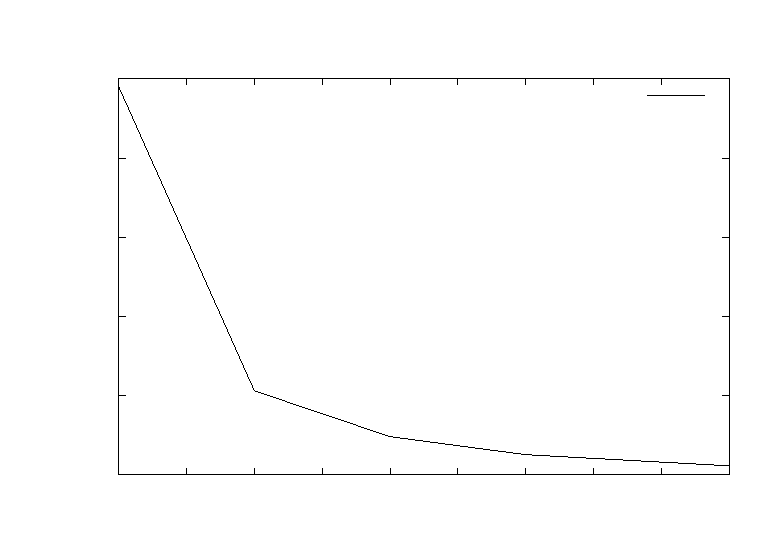
\includegraphics{graphs/scalability/swarm-scalability-waitingtime}}%
    \gplfronttext
  \end{picture}%
\endgroup
}
\caption{Average time in waiting state, $t_{wait}$, for each swarm density $c$, for the honey bee algorithm}
\label{fig:swarmscalabilitywaitingtime}
\end{figure}
%I'm here
However, the time spent by honey bee robots in the waiting state decreases as swarm density increases. This result is counter-intuitive, because an appropriately functioning division of labour mechanism would lead to an increase in average time in the waiting state as swarm density increases, due to increases in inter-robot interference. Further analysis is required in order to understand why the division of labour mechanism of the honey bee algorithm did not behave as expected. That said, the problem in the honey bee algorithm's division of labour mechanism does explain why the desert ant algorithm overtakes the honey bee algorithm for higher values of $c$: The honey bee algorithm is unable to regulate the number of active foragers for high values of $c$. The honey bee algorithm's recruitment mechanism is more exploitative than the site fidelity mechanism of the desert ant algorithm, which results in increased inter-robot interference when the honey bee algorithm fails to regulate the number of active foragers. The increased inter-robot interference for the honey bee algorithm for high values of $c$ results in a lower scalability than that of the desert ant algorithm.

\subsubsection{Problem scalability}
\label{results:problemscalability}

Figure~\ref{fig:problemscalability} plots the problem scalability performance measure, $S_p$ (described in Section~\ref{setup:problemscalability}), for each algorithm using the values given in Table~\ref{table:problemscalability}. The results present the macro performance measure, $S_p$, which is calculated over all experiments, for each value of $p$. The figure includes a plot of ``Expected scalability". The values for ``Expected scalability" were calculated based on the assumption that foraging efficiency would degrade directly proportional to the increase in problem complexity. The expected values for foraging efficiency at each problem complexity were used to calculate $S_p$ for ``Expected scalability". All algorithms outperformed the expected scalability and thus problem scalability for all algorithms is better than the expected scalability which is good. 


\begin{table}[!htbp]
    \centering
    \caption{Problem scalability, $S_{p_i}$, for each environment density, $p_i$, for each algorithm}
    \label{table:problemscalability}
    \begin{tabular}{@{}llllll@{}}
    \toprule
    \textbf{$p$}                  & \textbf{0.05} & \textbf{0.2        } & \textbf{0.5}         & \textbf{0.7}         & \textbf{0.9}         \\ \midrule
    \textbf{desert ant}           & 1    & 0.488 & 0.231 & 0.182 & 0.169 \\
    \textbf{honey bee}            & 1    & 0.602 & 0.283 & 0.217 & 0.196 \\
    \textbf{na\"ive}              & 1    & 0.502 & 0.257 & 0.195 & 0.175 \\
    \textbf{Expected} & 1    & 0.25        & 0.1         & 0.071 & 0.056 \\ \bottomrule
    \end{tabular}
\end{table}

According to Figure~\ref{fig:problemscalability}, the honey bee algorithm is the most scalable in terms of problem scalability, followed by the na\"ive algorithm, with the desert ant algorithm exhibiting the worst scalability.


\begin{figure}[!htbp]
    \centering
    \resizebox{\textwidth}{!}{% GNUPLOT: LaTeX picture with Postscript
\begingroup
  \makeatletter
  \providecommand\color[2][]{%
    \GenericError{(gnuplot) \space\space\space\@spaces}{%
      Package color not loaded in conjunction with
      terminal option `colourtext'%
    }{See the gnuplot documentation for explanation.%
    }{Either use 'blacktext' in gnuplot or load the package
      color.sty in LaTeX.}%
    \renewcommand\color[2][]{}%
  }%
  \providecommand\includegraphics[2][]{%
    \GenericError{(gnuplot) \space\space\space\@spaces}{%
      Package graphicx or graphics not loaded%
    }{See the gnuplot documentation for explanation.%
    }{The gnuplot epslatex terminal needs graphicx.sty or graphics.sty.}%
    \renewcommand\includegraphics[2][]{}%
  }%
  \providecommand\rotatebox[2]{#2}%
  \@ifundefined{ifGPcolor}{%
    \newif\ifGPcolor
    \GPcolorfalse
  }{}%
  \@ifundefined{ifGPblacktext}{%
    \newif\ifGPblacktext
    \GPblacktexttrue
  }{}%
  % define a \g@addto@macro without @ in the name:
  \let\gplgaddtomacro\g@addto@macro
  % define empty templates for all commands taking text:
  \gdef\gplbacktext{}%
  \gdef\gplfronttext{}%
  \makeatother
  \ifGPblacktext
    % no textcolor at all
    \def\colorrgb#1{}%
    \def\colorgray#1{}%
  \else
    % gray or color?
    \ifGPcolor
      \def\colorrgb#1{\color[rgb]{#1}}%
      \def\colorgray#1{\color[gray]{#1}}%
      \expandafter\def\csname LTw\endcsname{\color{white}}%
      \expandafter\def\csname LTb\endcsname{\color{black}}%
      \expandafter\def\csname LTa\endcsname{\color{black}}%
      \expandafter\def\csname LT0\endcsname{\color[rgb]{1,0,0}}%
      \expandafter\def\csname LT1\endcsname{\color[rgb]{0,1,0}}%
      \expandafter\def\csname LT2\endcsname{\color[rgb]{0,0,1}}%
      \expandafter\def\csname LT3\endcsname{\color[rgb]{1,0,1}}%
      \expandafter\def\csname LT4\endcsname{\color[rgb]{0,1,1}}%
      \expandafter\def\csname LT5\endcsname{\color[rgb]{1,1,0}}%
      \expandafter\def\csname LT6\endcsname{\color[rgb]{0,0,0}}%
      \expandafter\def\csname LT7\endcsname{\color[rgb]{1,0.3,0}}%
      \expandafter\def\csname LT8\endcsname{\color[rgb]{0.5,0.5,0.5}}%
    \else
      % gray
      \def\colorrgb#1{\color{black}}%
      \def\colorgray#1{\color[gray]{#1}}%
      \expandafter\def\csname LTw\endcsname{\color{white}}%
      \expandafter\def\csname LTb\endcsname{\color{black}}%
      \expandafter\def\csname LTa\endcsname{\color{black}}%
      \expandafter\def\csname LT0\endcsname{\color{black}}%
      \expandafter\def\csname LT1\endcsname{\color{black}}%
      \expandafter\def\csname LT2\endcsname{\color{black}}%
      \expandafter\def\csname LT3\endcsname{\color{black}}%
      \expandafter\def\csname LT4\endcsname{\color{black}}%
      \expandafter\def\csname LT5\endcsname{\color{black}}%
      \expandafter\def\csname LT6\endcsname{\color{black}}%
      \expandafter\def\csname LT7\endcsname{\color{black}}%
      \expandafter\def\csname LT8\endcsname{\color{black}}%
    \fi
  \fi
    \setlength{\unitlength}{0.0500bp}%
    \ifx\gptboxheight\undefined%
      \newlength{\gptboxheight}%
      \newlength{\gptboxwidth}%
      \newsavebox{\gptboxtext}%
    \fi%
    \setlength{\fboxrule}{0.5pt}%
    \setlength{\fboxsep}{1pt}%
\begin{picture}(7200.00,5040.00)%
    \gplgaddtomacro\gplbacktext{%
      \csname LTb\endcsname%
      \put(740,640){\makebox(0,0)[r]{\strut{}$0$}}%
      \put(740,1020){\makebox(0,0)[r]{\strut{}$0.1$}}%
      \put(740,1400){\makebox(0,0)[r]{\strut{}$0.2$}}%
      \put(740,1780){\makebox(0,0)[r]{\strut{}$0.3$}}%
      \put(740,2160){\makebox(0,0)[r]{\strut{}$0.4$}}%
      \put(740,2540){\makebox(0,0)[r]{\strut{}$0.5$}}%
      \put(740,2919){\makebox(0,0)[r]{\strut{}$0.6$}}%
      \put(740,3299){\makebox(0,0)[r]{\strut{}$0.7$}}%
      \put(740,3679){\makebox(0,0)[r]{\strut{}$0.8$}}%
      \put(740,4059){\makebox(0,0)[r]{\strut{}$0.9$}}%
      \put(740,4439){\makebox(0,0)[r]{\strut{}$1$}}%
      \put(860,440){\makebox(0,0){\strut{}$0$}}%
      \put(1524,440){\makebox(0,0){\strut{}$0.1$}}%
      \put(2189,440){\makebox(0,0){\strut{}$0.2$}}%
      \put(2853,440){\makebox(0,0){\strut{}$0.3$}}%
      \put(3517,440){\makebox(0,0){\strut{}$0.4$}}%
      \put(4182,440){\makebox(0,0){\strut{}$0.5$}}%
      \put(4846,440){\makebox(0,0){\strut{}$0.6$}}%
      \put(5510,440){\makebox(0,0){\strut{}$0.7$}}%
      \put(6175,440){\makebox(0,0){\strut{}$0.8$}}%
      \put(6839,440){\makebox(0,0){\strut{}$0.9$}}%
    }%
    \gplgaddtomacro\gplfronttext{%
      \csname LTb\endcsname%
      \put(160,2539){\rotatebox{-270}{\makebox(0,0){\strut{}Problem Scalability ($PS$)}}}%
      \put(3849,140){\makebox(0,0){\strut{}Environment Density ($p$)}}%
      \put(3849,4739){\makebox(0,0){\strut{}Problem Scalability, $PS$, for each environment density $p$, for each algorithm}}%
      \put(5936,4276){\makebox(0,0)[r]{\strut{}Na\"ive}}%
      \put(5936,4076){\makebox(0,0)[r]{\strut{}Desert Ant}}%
      \put(5936,3876){\makebox(0,0)[r]{\strut{}Honey Bee}}%
      \put(5936,3676){\makebox(0,0)[r]{\strut{}Expected Scalability}}%
    }%
    \gplbacktext
    \put(0,0){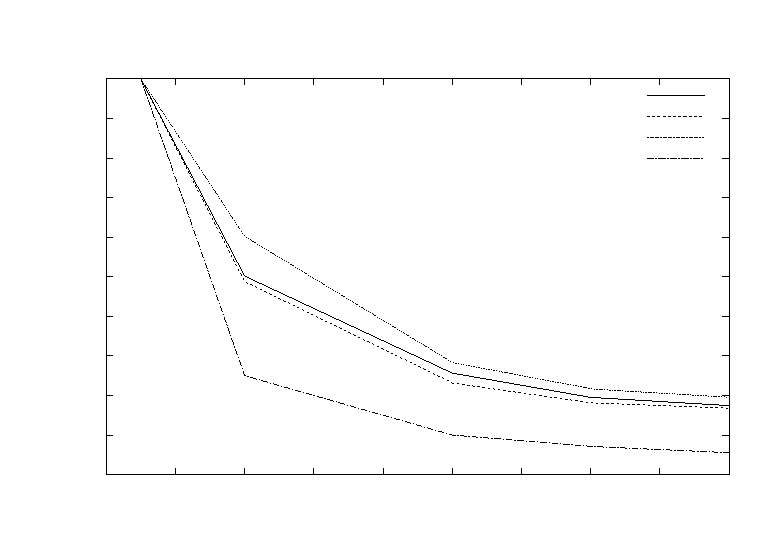
\includegraphics{chapters/chapter6/graphs/scalability/problemscalability}}%
    \gplfronttext
  \end{picture}%
\endgroup
}
    \caption{Problem Scalability, $S_p$, for each environment density $p_i$, for each algorithm}
    \label{fig:problemscalability}
\end{figure}
    

In order to explain the reason for this, consider the following rational argument: The desert ant algorithm differs from the na\"ive algorithm in only one aspect: The desert ant algorithm employs site fidelity and the na\"ive algorithm does not. The site fidelity (discussed in Section~\ref{desertantforaging}) enables a robot to return to a previously foraged site. The desert ant algorithm's use of site fidelity must, directly or indirectly, be the reason that the na\"ive algorithm is more scalable than the desert ant algorithm. To understand why the site fidelity mechanism is negatively influencing scalability, consider the following scenario: A desert ant robot employs a random walk through a complex environment, as shown by the dashed line in Figure~\ref{fig:desertantsitefidelity}. The random walk leads the desert ant robot to a hard-to-reach source of prioritized items. The desert ant robot stores the PI vector, shown by the solid line on the figure, which is needed to return back to the site after offloading the loaded item at the sink. The next time the desert ant wants to return to the previous site, the robot will still need to perform the same obstacle avoidance in order to navigate around the obstacles to return to the previously foraged site, since the PI vector only consists of an overall heading and distance to the site. As is evident in Figure~\ref{fig:desertantsitefidelity}, there may exist an easier to reach site for prioritized items, but the desert ant robot will waste time by continuing to forage the hard to locate source of items. The na\"ive algorithm will not try to return to the hard to find site and is more likely to randomly find the prioritized resource site that is nearer to the sink (indicated by the dotted line), and thus the time taken to forage a single item will be faster, and so foraging efficiency will be increased. The time spent on relocating hard to access sites in more complex environments can slow the desert ant algorithm down. The na\"ive algorithm benefits from a more complex environment, because there will be lots of items to find nearer to the sink that do not require any complex search to relocate. 

\begin{figure}[!htbp]
    \centering
    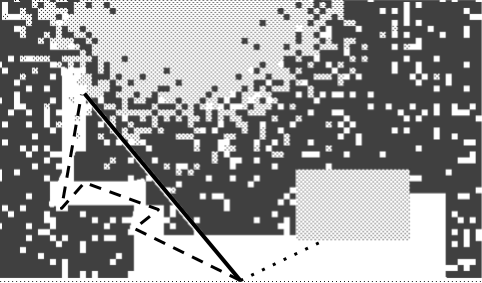
\includegraphics[width=0.75\textwidth]{figures/problem-scalability-desertant2.png}
    \caption{Illustration of the inefficiencies of the desert ant algorithm's site fidelity in dense environments. Solid areas are non-prioritized items, white areas are free cells, and shaded areas are prioritized items. The dashed path is a hypothetical random walk performed by a robot, the solid path is the PI vector for the dashed random walk, and the dotted path is an alternative random walk.}
    \label{fig:desertantsitefidelity}
\end{figure}

Additionally, in environments that are more dense, all desert ant robots are more likely to locate the same high density area. The more dense the area, the more robots will try to forage the same area and the more inter-robot and environmental interference will occur. The desert ant robots try to exploit the same high density areas. On the other hand, the na\"ive algorithm will explore more. Thus the na\"ive algorithm will experience less inter-robot and environmental interference as a result. 


The honey bee algorithm uses site fidelity, and also communicates those sites to others. Despite the use of a site fidelity mechanism, similar to the desert ant algorithm, the honey bee algorithm is the most scalable. The reason why the site fidelity of the honey bee algorithm does not impact on the scalability can be attributed the ability of the honey bee algorithm to adapt the swarm specialization ratio, $\tau$, to focus on foraging dense areas of obstacles, rather than having to expensively navigate around the obstacles. The ability of the honey bee algorithm to concentrate on clearing obstacles in highly dense environments will increase overall ease of access to the high quality sites, as discovered in Section~\ref{results:flexibility:environmentdistribution}. Thus efficiency of the honey bee algorithm in highly dense environments is improved. Therefore, the honey bee algorithm is the most scalable in terms of the problem complexity.



\subsection{Robustness}
\label{results:robustness}
% describe fault tolerance, and provide rational arguments as to why it would be more or less 
As discussed in Section~\ref{robustness}, robot swarms achieve robustness by exhibiting the properties of redundancy, multiplicity of sensing, and decentralized coordination. This study does not perform an empirical robustness study to specifically address how fault tolerant each algorithm is. Instead, this section provides rational arguments supported by empirical evidence to discuss each algorithm's robustness. Section~\ref{results:redundancy} discusses robustness in terms of the resulting redundancy of each of the algorithms, and Section~\ref{results:decentralizedcoordination} discusses robustness in terms of decentralized coordination.

\subsubsection{Redundancy}
\label{results:redundancy}

As discussed in Section~\ref{robustness}, redundancy in a swarm is achieved by giving all, or a portion of the robots in the swarm the same capabilities. In this way, if a percentage of the swarm malfunctions, the other robots have the capability to take the malfunctioning robots' place. A swarm demonstrates the highest level of redundancy when any robot can take on the role of any other robot that malfunctions in a swarm. 

For each of our experiments, each swarm is configured with an initial swarm specialization ratio (as discussed in Chapter~\ref{chap:experiment}) to enable a portion of robots to forage prioritized items and the another portion to forage non-prioritized items. 

If a portion of robots in a swarm malfunctions or are destroyed, then the swarm specialization ratio will be affected. As shown in Section~\ref{results:flexibility}, the foraging efficiency of the na\"ive and desert ant algorithms were effected by the initial swarm specialization ratio $\tau$. It follows that, if the swarm specialization ratio is unexpectedly changed during the swarm experiment, a change in the foraging efficiency of the swarm would persist for the experiment. In particular, consider the following extreme scenarios: Suppose that all the robots which were foraging for prioritized items (for some $\tau > 0$) are destroyed or malfunction (thus $\tau=0$). Foraging efficiency would drop to 0, because no robots exist to forage prioritized items. Similarly, consider an environment where all prioritized items are blocked by non-prioritized items and that $\tau < 1$. If all non-prioritized robots suffer a malfunction or are destroyed, then $\tau=1$ and no robots will be available to forage non-prioritized items. Foraging efficiency, $E_P$, will then drop to 0. 

As shown in Section~\ref{results:flexibility}, the honey bee algorithm experiences little change to efficiency when $\tau(0)$ is varied. The honey bee algorithm adapts the swarm specialization ratio  over time. It follows that, for the above scenarios, the honey bee algorithm will be able to re-adapt the swarm specialization ratio in order to replenish the robots that were destroyed. 

The robots controlled by the honey bee algorithm are homogeneous, in that every robot in the swarm has the ability to take on any of the roles required for the algorithm to function (i.e. scout, unemployed forager, employed forager), as well as to adapt to forage either prioritized or non-prioritized items. It follows that the swarms running the honey bee algorithm are more redundant than swarms running the desert ant algorithm and the na\"ive algorithm.

\subsubsection{Decentralized Coordination}
\label{results:decentralizedcoordination}

Decentralized coordination can be attained by creating algorithms that do not depend on decisions, actions, or sensor readings of any single individual or a few individuals of the swarm. This section provides rational arguments to compare the decentralized coordination mechanisms for each algorithm, supported by evidence. 

The robots of both the desert ant algorithm and na\"ive algorithm do not depend on each other and there is no explicit coordination mechanism. Despite no explicit coordination mechanism existing between robots in the desert ant and na\"ive swarms, the robots coordinate implicitly by using obstacle avoidance to avoid obstructing each other's movement. In that way, the robots in the swarm attempt to avoid inter-robot interference. The mechanism for obstacle avoidance is entirely decentralized, because each robot only depends on its own internal sensors and thus coordination is entirely decentralized.

On the other hand, the honey bee algorithm uses explicit communication as a coordination mechanism in order to recruit foragers to areas with a high density of prioritized items (as described in Section~\ref{honeybeeforaging}). If the scout robots experience a fault in evaluating the quality of a site (for example, a robot detects that a site is of high quality when it is actually a site of poor quality), then foragers will be incorrectly recruited to forage sites of low quality. Only a few individuals (the scouts) can coordinate the swarm and therefore any faults in the scout robots may negatively influence the efficiency of the entire swarm. The coordination mechanism of the honey bee algorithm is not entirely decentralized and the honey bee algorithm is less robust than both the desert ant algorithm and the na\"ive algorithm in terms of decentralized coordination.

To provide further evidence that the scout robots can mislead the swarm to incorrectly forage areas that have low quality resources, an examination of the average time spent in the recruitment state, per item foraged, per robot has been done. Table~\ref{averagetimerecruitment} and Figure~\ref{fig:recruitmenttime} illustrate the average time steps, $t_{recruitment}$, spent performing recruitment per robot, per (both prioritized and non-prioritized) item foraged for the honey bee algorithm, for each environment distribution. The results were averaged over each environment item type ratio, $r$. 

\begin{table}[!htbp]
\centering
\caption{Average time steps, per robot, per prioritized item foraged, that were spent performing recruitment for the honey bee algorithm, in each environment distribution, for each environment item type ratio $r$.}
\label{averagetimerecruitment}
\begin{tabular}{@{}lllll@{}}
\toprule
$r$            & \textbf{Clustered} & \textbf{Gaussian} & \textbf{Uniform} & \textbf{Vein} \\ \midrule
\textbf{0}        & 0        & 0       & 0      & 0   \\
\textbf{0.2}      & 0.119        & 0.152       & 0.120       & 0.161   \\
\textbf{0.25}     & 0.127        & 0.144       & 0.128      & 0.159   \\
\textbf{0.33} & 0.140        & 0.135       & 0.139      & 0.152   \\
\textbf{0.5}      & 0.162        & 0.157        & 0.163       & 0.169   \\
\textbf{0.67} & 0.182        & 0.175       & 0.183      & 0.152   \\
\textbf{0.75}     & 0.179        & 0.177       & 0.184      & 0.172   \\
\textbf{0.8}      & 0.183        & 0.183       & 0.186      & 0.191   \\
\textbf{1}        & 0.167        & 0.173       & 0.163      & 0.219   \\ \bottomrule
\end{tabular}
\end{table}


\begin{figure}[!htbp]
\centering
\resizebox{\textwidth}{!}{% GNUPLOT: LaTeX picture with Postscript
\begingroup
  \makeatletter
  \providecommand\color[2][]{%
    \GenericError{(gnuplot) \space\space\space\@spaces}{%
      Package color not loaded in conjunction with
      terminal option `colourtext'%
    }{See the gnuplot documentation for explanation.%
    }{Either use 'blacktext' in gnuplot or load the package
      color.sty in LaTeX.}%
    \renewcommand\color[2][]{}%
  }%
  \providecommand\includegraphics[2][]{%
    \GenericError{(gnuplot) \space\space\space\@spaces}{%
      Package graphicx or graphics not loaded%
    }{See the gnuplot documentation for explanation.%
    }{The gnuplot epslatex terminal needs graphicx.sty or graphics.sty.}%
    \renewcommand\includegraphics[2][]{}%
  }%
  \providecommand\rotatebox[2]{#2}%
  \@ifundefined{ifGPcolor}{%
    \newif\ifGPcolor
    \GPcolorfalse
  }{}%
  \@ifundefined{ifGPblacktext}{%
    \newif\ifGPblacktext
    \GPblacktexttrue
  }{}%
  % define a \g@addto@macro without @ in the name:
  \let\gplgaddtomacro\g@addto@macro
  % define empty templates for all commands taking text:
  \gdef\gplbacktext{}%
  \gdef\gplfronttext{}%
  \makeatother
  \ifGPblacktext
    % no textcolor at all
    \def\colorrgb#1{}%
    \def\colorgray#1{}%
  \else
    % gray or color?
    \ifGPcolor
      \def\colorrgb#1{\color[rgb]{#1}}%
      \def\colorgray#1{\color[gray]{#1}}%
      \expandafter\def\csname LTw\endcsname{\color{white}}%
      \expandafter\def\csname LTb\endcsname{\color{black}}%
      \expandafter\def\csname LTa\endcsname{\color{black}}%
      \expandafter\def\csname LT0\endcsname{\color[rgb]{1,0,0}}%
      \expandafter\def\csname LT1\endcsname{\color[rgb]{0,1,0}}%
      \expandafter\def\csname LT2\endcsname{\color[rgb]{0,0,1}}%
      \expandafter\def\csname LT3\endcsname{\color[rgb]{1,0,1}}%
      \expandafter\def\csname LT4\endcsname{\color[rgb]{0,1,1}}%
      \expandafter\def\csname LT5\endcsname{\color[rgb]{1,1,0}}%
      \expandafter\def\csname LT6\endcsname{\color[rgb]{0,0,0}}%
      \expandafter\def\csname LT7\endcsname{\color[rgb]{1,0.3,0}}%
      \expandafter\def\csname LT8\endcsname{\color[rgb]{0.5,0.5,0.5}}%
    \else
      % gray
      \def\colorrgb#1{\color{black}}%
      \def\colorgray#1{\color[gray]{#1}}%
      \expandafter\def\csname LTw\endcsname{\color{white}}%
      \expandafter\def\csname LTb\endcsname{\color{black}}%
      \expandafter\def\csname LTa\endcsname{\color{black}}%
      \expandafter\def\csname LT0\endcsname{\color{black}}%
      \expandafter\def\csname LT1\endcsname{\color{black}}%
      \expandafter\def\csname LT2\endcsname{\color{black}}%
      \expandafter\def\csname LT3\endcsname{\color{black}}%
      \expandafter\def\csname LT4\endcsname{\color{black}}%
      \expandafter\def\csname LT5\endcsname{\color{black}}%
      \expandafter\def\csname LT6\endcsname{\color{black}}%
      \expandafter\def\csname LT7\endcsname{\color{black}}%
      \expandafter\def\csname LT8\endcsname{\color{black}}%
    \fi
  \fi
    \setlength{\unitlength}{0.0500bp}%
    \ifx\gptboxheight\undefined%
      \newlength{\gptboxheight}%
      \newlength{\gptboxwidth}%
      \newsavebox{\gptboxtext}%
    \fi%
    \setlength{\fboxrule}{0.5pt}%
    \setlength{\fboxsep}{1pt}%
\begin{picture}(7200.00,5040.00)%
    \gplgaddtomacro\gplbacktext{%
      \csname LTb\endcsname%
      \put(860,640){\makebox(0,0)[r]{\strut{}$0$}}%
      \put(860,1472){\makebox(0,0)[r]{\strut{}$0.05$}}%
      \put(860,2304){\makebox(0,0)[r]{\strut{}$0.1$}}%
      \put(860,3135){\makebox(0,0)[r]{\strut{}$0.15$}}%
      \put(860,3967){\makebox(0,0)[r]{\strut{}$0.2$}}%
      \put(860,4799){\makebox(0,0)[r]{\strut{}$0.25$}}%
      \put(980,440){\makebox(0,0){\strut{}$0$}}%
      \put(2152,440){\makebox(0,0){\strut{}$0.2$}}%
      \put(3324,440){\makebox(0,0){\strut{}$0.4$}}%
      \put(4495,440){\makebox(0,0){\strut{}$0.6$}}%
      \put(5667,440){\makebox(0,0){\strut{}$0.8$}}%
      \put(6839,440){\makebox(0,0){\strut{}$1$}}%
    }%
    \gplgaddtomacro\gplfronttext{%
      \csname LTb\endcsname%
      \put(160,2719){\rotatebox{-270}{\makebox(0,0){\strut{}$t_{recruitment}$}}}%
      \put(3909,140){\makebox(0,0){\strut{}Environment item type ratio ($r$)}}%
      \put(5936,4636){\makebox(0,0)[r]{\strut{}clustered}}%
      \put(5936,4436){\makebox(0,0)[r]{\strut{}gaussian}}%
      \put(5936,4236){\makebox(0,0)[r]{\strut{}uniform}}%
      \put(5936,4036){\makebox(0,0)[r]{\strut{}vein}}%
    }%
    \gplbacktext
    \put(0,0){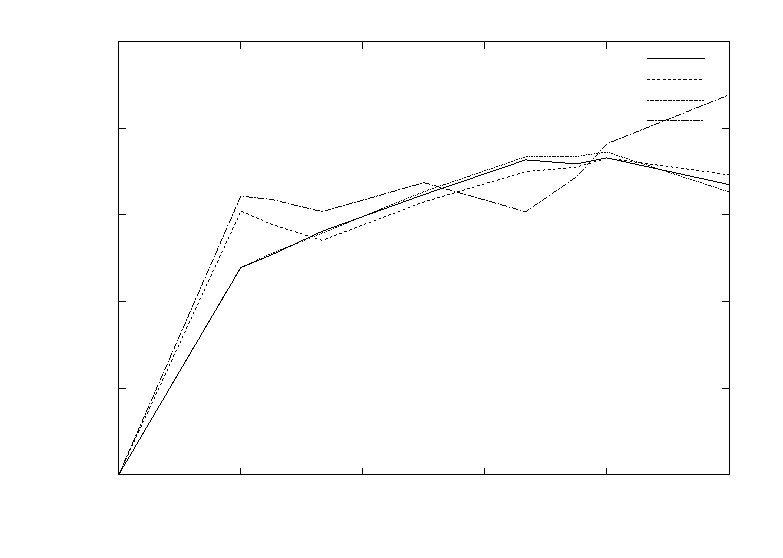
\includegraphics{graphs/robustness/robustness-recruitment-type-honeybee}}%
    \gplfronttext
  \end{picture}%
\endgroup
}
\caption{Average time steps spent performing recruitment activities by robots of the swarm for each item foraged, $t_{recruitment}$, for the honey bee algorithm, per item distribution, for each environment item type ratio, $r$.}
\label{fig:recruitmenttime}
\end{figure}

Table~\ref{averagetimerecruitment} illustrates that, on average, each robot spent at least 11.96\% of its total foraging time recruiting other robots to forage higher quality areas for all values of $r > 0$. This is particularly relevant for uniformly distributed environments with a low ratio of prioritized items ($r = 0.2$), because it is unlikely that sites of high quality do not exist, because the prioritized items will be scarce and scattered. This means that the scouts were recruiting other robots to forage areas that were not of a high quality. The fact that scouts can mislead the swarm to foraging sites with low quality, demonstrates that the honey bee algorithm is less robust due to less decentralized coordination.

%%%%%%%%%%%%%%%%%%%%%%%%%%%%%%%%%%%%%%%%%%%%%%%%%
%%%%%%%%%%%%%%%%%%%%%%%%%%%%%%%%%%%%%%%%%%1%%%%%%%


\section{Conclusions}
\label{Conclusions}

The first contribution of this research was the introduction of a novel variation of the swarm robotics multi-foraging problem, denoted as the prioritized foraging problem. The prioritized foraging problem differs from other multi-foraging swarm robotics problems in that two types of items which have different priorities exist. The items with higher priorities should be foraged as fast as possible, while the non-prioritized items should only be foraged to enable the prioritized items to be foraged at a faster rate. The prioritized foraging problem is a novel way of modelling the real-world problem of search and rescue.  

Existing na\"ive and desert ant algorithms were reviewed and selected for evaluation on the prioritized foraging problem. Furthermore, a novel honey bee inspired foraging algorithm was developed, which specifically modelled the recruitment mechanism and division of labour mechanism of honey bee swarms.

Emperical experiments were defined in Chapter~\ref{chap:experiment}, and an emperical analysis was performed in Chapter~\ref{chap:results}. The purpose of the emperical analysis was to investigate each algorithm's performance on the prioritized foraging problem in terms of the major swarm robotics characteristics of efficiency, scalability, flexibility, and robustness as well as the behaviours that enabled those characteristics. 

Each algorithm's efficiency was compared to each other algorithm's efficency using a wins and losses approach. Results showed that the honey bee algorithm was the most efficient over all environments and swarm configurations, while the desert ant was the next most efficient and the na\"ive algorithm was the least efficient.

The flexibility of the algorithms was analysed in terms of the flexibility over environmental item ratio, and the flexibility over different environment distribution types. Results indicated that the honey bee algorithm could adapt the swarm's specialization ratio to effectively forage a given environment item ratio, and was therefore the most flexible in terms of environmental item ratio. The na\"ive algorithm only appeared more flexible than the desert ant algorithm because the na\"ive algorithm performed equally poorly across all environment item distributions, where as the desert algorithm favoured particular item distributions.

The honey bee algorithm was the most flexible over different types of environmental distributions, followed by the desert ant algorithm, and lastly the na\"ive algorithm. The honey bee algorithm's high flexibility was attributed to its adaptation of the specialization ratio to better suit the environment ratio of the accessible environment. The honey bee algorithm's adaptation of specialization ratio allowed the swarm to focus on foraging non-prioritized items when only non-prioritized items were accessible, and then to adjust the ratio to focus on foraging prioritized items when more prioritized items became accessible, and vice versa. The desert ant and na\"ive algorithms were less flexible than the honey bee algorithm, due to their inability to adapt the initial swarm specialization ratio.

The scalability of each algorithm was analyzed in terms of swarm scalability and problem scalability. Swarm scalability was sub-linear for all algorithms, however the na\"ive algorithm was the most scalable. The desert ant algorithm had poor swarm scalability when compared to the na\"ive algorithm. The desert ant algorithm's site fidelity increased inter-robot interference, which resulted in decreased efficiency when swarm density was high. The honey bee algorithm was shown to be slightly more scalable than the desert ant algorithm, due to the honey bee algorithm's attempt to regulate the number of active foragers by division of labour. Future investigation is necessary to determine why the honey bee algorithm did not regulate the number of foragers at high swarm densities very well. 

The honey bee algorithm was the most scalable in terms of the problem density, followed by the na\"ive algorithm, and lastly the desert ant algorithm. The desert ant algorithm performed comparatively better than the na\"ive algorithm in terms of problem scalability. It was theorized that the desert ant algorithm could potentially exploit hard to reach sites in complex environments. The problem scalability of the honey bee algorithm was attributed the honey bee algorithm's ability to adapt the swarm specialization ratio to help clear non-prioritized items. By clearing the non-prioritized items, the honey bee algorithm decreased inter-robot and environmental interference, which in turn increased the foraging efficiency in problems of high complexity.

Lastly, the robustness of each algorithm was evaluated in terms of redundancy and decentralized coordination. A rational argument  motivated that the honey bee algorithm was the most redundant, because the honey bee algorithm swarm is completely homogeneous. The robots of the desert ant algorithm and na\"ive algorithm are heterogeneous, and thus the swarm is less redudant. The coordination between robots of the desert ant and na\"ive algorithms was determined to be more decentralized than the coordination of robots in the honey bee algorithm. Evidence showed that invalid information was communicated to the rest of swarm by individuals with faulty information, impacting efficiency and showing that communication is less decentralized.

In summation, this dissertation primarily contributed the prioritized foraging problem and the novel honey bee inspired foraging swarm robotic algorithm. The emperical analysis provided a detailed view of how well each algorithm embodied each major characteristic of swarm robotics on the prioritized foraging problem.

\bibliographystyle{elsarticle-num} 
\bibliography{journal}
    
    %% else use the following coding to input the bibitems directly in the
    %% TeX file.
    
    %\begin{thebibliography}{}
    
    %% \bibitem{label}
    %% Text of bibliographic item
    
    %\bibitem{}
    
   % \end{thebibliography}
    \end{document}
    \endinput
    %%
    %% End of file `elsarticle-template-num.tex'.
    